% ============================================================
%  股票特征建模与买入时机研究 — LaTeX 实验报告
%  编译: xelatex 实验报告.tex (×2)
% ============================================================
\documentclass[12pt,a4paper]{ctexart}

% ---------- 页面 ----------
\usepackage{xcolor}
\usepackage[top=2.54cm, bottom=2.54cm, left=3.18cm, right=3.18cm]{geometry}
\usepackage{setspace}
\onehalfspacing

% ---------- 图表 ----------
\usepackage{graphicx}
\usepackage{float}
\usepackage{booktabs}
\usepackage{multirow}
\usepackage{array}
\usepackage{tabularx}
\usepackage{longtable}
\newcolumntype{Y}{>{\centering\arraybackslash}X}
\newcolumntype{L}[1]{>{\raggedright\arraybackslash}p{#1}}
\newcolumntype{C}[1]{>{\centering\arraybackslash}p{#1}}

% ---------- 数学 ----------
\usepackage{amsmath,amssymb}
\usepackage{bm}

% ---------- 超链接 ----------
\usepackage[colorlinks=true,linkcolor=black,citecolor=black,urlcolor=blue]{hyperref}

% ---------- 其他 ----------
\usepackage{enumitem}
\usepackage{caption}
\usepackage{fancyhdr}
\usepackage{tocloft}

% ---------- 编号 ----------
\numberwithin{figure}{section}
\numberwithin{table}{section}
\setcounter{tocdepth}{3}

% ---------- 页眉页脚 ----------
\pagestyle{fancy}
\fancyhf{}
\fancyfoot[C]{\thepage}
\renewcommand{\headrulewidth}{0pt}

\begin{document}

\begin{titlepage}
\centering
\vspace*{3cm}
{\heiti\fontsize{26pt}{36pt}\selectfont 电\ 子\ 科\ 技\ 大\ 学\ 实\ 验\ 报\ 告}
\vspace{2.5cm}

\begin{tabular}{rl}
{\heiti 课程名称：} & 数学实验 \hspace{2.5cm} {\heiti 实验地点：} 科A \\[8pt]
{\heiti 指导教师：} & 李佑铭 \hspace{2.5cm} {\heiti 评\quad 分：} \\[8pt]
\end{tabular}

\vspace{2cm}

{\heiti\large 完成实验学生信息：}

\vspace{0.3cm}
{\small\color{gray} 学生人数按照任课教师要求限定；对于"评价、改进、总结和体会"\\都要认真填写，和其他内容是评价实验成绩的重要参考。}

\vspace{0.5cm}
\begin{tabularx}{\textwidth}{c c c c c X}
\toprule
序 & 姓名 & 学号 & 选课序号 & 贡献百分比(\%) & 备注 \\
\midrule
1 & 毕博昊 & 2025080901001 &  & 100 & 全部代码编写、实验设计、报告撰写 \\
\bottomrule
\end{tabularx}
\end{titlepage}

% ============================================================
\newpage
\section*{摘要}
\addcontentsline{toc}{section}{摘要}

本文基于 A 股市场 200 只股票日线数据（2024.11—2026.03），提取 MA、MACD、RSI、KDJ、箱体位置等 20+ 维技术特征，设计了四个差异化买入策略（追涨型、低吸型、超跌型、精选型），在 8 个持有周期上完成全样本回测（计入佣金、印花税、滑点成本）。核心结论：箱体底部反弹策略最优（60 天胜率 70.2\%，净收益 9.19\%，夏普 7.38），"低买"逻辑显著优于"追涨"（全部策略 $p < 0.001$）。

\vspace{0.5cm}
\noindent{\bfseries 关键词：} 量化交易；技术指标；买入策略；回测；夏普比率；箱体策略

\newpage
\tableofcontents
\newpage

% ============================================================
\section{实验完成情况说明}

\subsection*{表1\quad 自己做的工作}
\begin{center}
\small
\begin{tabularx}{\textwidth}{c X L{4.5cm}}
\toprule
序号 & \centering 自己做的工作 & 备注（技术细节） \\
\midrule
1 & 设计了完整的 5 阶段量化策略研究流水线（数据加载→特征计算→信号生成→回测→可视化），使用 MATLAB R2025b 实现全部模块 & 实现了 15 个函数文件 \\
\addlinespace
2 & 实现了 20+ 维技术指标的特征工程（MA/MACD/RSI/KDJ/箱体位置/均线交叉/成交量均比），全部采用递推/向量化实现 & MA 用 movmean；MACD 用递推 EMA；RSI 用 Wilders smoothing；KDJ 用递推公式 \\
\addlinespace
3 & 独立设计并实现了 4 个差异化买入策略（追涨型、低吸型、超跌型、精选型），覆盖不同的市场逻辑 & 形成完整对照实验 \\
\addlinespace
4 & 实现了含交易摩擦成本的完整回测引擎：佣金（万分之三双向）+ 印花税（千分之0.5 卖出）+ 滑点（1bp 双向）+ 最低佣金（5元） & 单笔净收益 = 毛收益 $-$ 成本 \\
\addlinespace
5 & 计算了风险调整绩效指标（夏普比率年化、最大回撤、卡玛比率、盈亏比）和统计显著性检验（二项检验 + Bootstrap 10,000 次 95\% CI） & $H_0$: 胜率=50\% \\
\addlinespace
6 & 完成了 MATLAB + Python 双引擎实现，200 只股票全流程回测，产出 CSV/Excel/可视化图表，撰写正式实验报告 & 5 张 PNG + 2 份数据文件 \\
\bottomrule
\end{tabularx}
\end{center}

\subsection*{表2\quad 使用AI做的工作}
\begin{center}
\small
\begin{tabularx}{\textwidth}{c X L{4.8cm}}
\toprule
序号 & \centering 基于AI所做工作主题 & 备注 \\
\midrule
1 & Python stock\_strategy 代码初始框架生成与特征计算函数实现（RSI/KDJ 的 Wilder 平滑递推逻辑） & 基于任务提示词由大模型生成，人工核对验证所有数学公式 \\
\addlinespace
2 & Python→MATLAB 代码全量翻译（约 1500 行 Python→15 个.m 文件） & 逐模块转换，人工核对每行逻辑、修复维度不匹配和索引 bug \\
\addlinespace
3 & 可视化图表代码生成（hold\_period\_comparison / heatmap / sensitivity / significance\_forest 共 5 张图） & MATLAB exportgraphics 导出 PNG，人工调整布局色彩 \\
\addlinespace
4 & 实验报告初稿框架与数据表格填充 & 人工核对并修正所有数值、结论和公式 \\
\bottomrule
\end{tabularx}
\end{center}

\vspace{0.3cm}
{\small 注：表1用于说明自己主要做了哪些工作。表2用于说明AI辅助做了哪些工作。}

% ============================================================
\section{问题重述}

\subsection{实验背景}
股票市场中的交易决策高度依赖于对历史数据的建模与分析。通过对日线数据提取有效特征（如技术指标、趋势特征），可以构建量化交易策略，辅助判断买入时机。本实验要求从A股市场大量日线数据出发，完成从特征提取到策略设计与验证的完整流程。

\subsection{实验数据}
数据来源：tushare 库，200 只 A 股（深市+沪市），2024-11-11 至 2026-03-19，平均每只约 323 个交易日。字段：日期、股票代码、OHLCV、振幅、涨跌幅、涨跌额、换手率。

\subsection{实验任务}
\begin{enumerate}[leftmargin=*]
    \item {\bfseries 任务1：} 建立股票日线数据特征，并设计算法提取特征。给出后续交易策略需要用到的指标的计算方法、数学表达式和算法。主要考虑 MACD、RSI、KDJ、换手率、箱体指标。
    \item {\bfseries 任务2：} 设计交易策略（买入策略）。利用任务1得到的特征设计买入信号规则。信号日在第 $i$ 天，买入日为第 $i+1$ 天，持有 $H$ 个交易日后以收盘价卖出。
    \item {\bfseries 任务3：} 模型评估。对 200 只历史股票评估持有 $H=5,10,15,20,30,40,50,60$ 天的预测准确率、收益率等指标，以表格形式呈现实验结果。
\end{enumerate}

% ============================================================
\section{问题分析}

\subsection{特征提取分析}
日线数据提供 OHLCV 基础信息，但原始数据难以直接捕捉市场趋势。需通过数学变换提取五类技术特征：
\begin{itemize}[leftmargin=*]
    \item {\bfseries 趋势类：} MA（移动均线反映价格的中长期方向）
    \item {\bfseries 动量类：} MACD（揭示趋势强度和方向变化）、RSI（衡量超买超卖状态）
    \item {\bfseries 波动类：} KDJ（对短期价格波动敏感，辅助判断拐点）
    \item {\bfseries 位置类：} 箱体特征（量化当前价格在历史区间中的相对位置）
    \item {\bfseries 量能类：} 成交量均比（反映量价配合程度）
\end{itemize}

\subsection{策略设计分析}
四种策略覆盖不同的市场逻辑，形成完整对照实验：
\begin{itemize}[leftmargin=*]
    \item {\bfseries 追涨型（均线金叉+量能确认）：} 捕捉趋势启动点，辅以量能过滤假突破
    \item {\bfseries 低吸型（箱体底部反弹）：} 在阶段底部等待反转，安全性相对较高
    \item {\bfseries 超跌型（连跌反弹）：} 利用过度恐慌后的均值回归，信号密集
    \item {\bfseries 精选型（多指标共振）：} 多重条件过滤，以质量换数量
\end{itemize}

\subsection{评估方法分析}
从三个维度综合评估：
\begin{itemize}[leftmargin=*]
    \item {\bfseries 收益维度：} 胜率、平均收益率——赚不赚钱
    \item {\bfseries 风险维度：} 夏普比率、最大回撤、盈亏比——风险调整后是否划算
    \item {\bfseries 统计维度：} 二项检验 $p$ 值、Bootstrap 95\% CI——是否显著优于随机 50\%
\end{itemize}

% ============================================================
\section{模型假设}

\begin{enumerate}[leftmargin=*]
    \item {\bfseries 数据完整性假设：} 假设 CSV 数据中的价格和成交量数据真实反映市场交易情况。
    \item {\bfseries 无未来信息泄露：} 所有特征计算严格使用当前及历史数据，信号日在 $i$，买入日在 $i+1$。
    \item {\bfseries 流动性假设：} 假设每笔交易以收盘价成交，不考虑大单对市场的冲击（已用滑点 1 bp 近似补偿）。
    \item {\bfseries 独立资金假设：} 每笔交易视为独立事件，隐含无限资金和无资金占用约束——这适合做策略间的横向比较。
    \item {\bfseries 无分红调整假设：} 不考虑现金分红对价格的影响。
    \item {\bfseries 幸存者偏差：} 样本中的股票均为 2024--2026 年存续的股票，不含在此期间退市的股票，策略收益可能被高估。
\end{enumerate}

% ============================================================
\section{定义与符号说明}

\subsection{名词解释}
\begin{itemize}[leftmargin=*]
    \item {\bfseries 移动均线 (MA)：} 过去 $N$ 个交易日收盘价的算术平均值。
    \item {\bfseries 金叉：} 短期均线从下方上穿长期均线，视为买入参考信号。
    \item {\bfseries MACD：} 指数平滑异同移动平均线，由快慢 EMA 差值构成。
    \item {\bfseries RSI：} 相对强弱指数，使用 Wilders smoothing（$\alpha=1/14$），衡量价格变动的速度和幅度。
    \item {\bfseries KDJ：} 随机指标，由 K、D、J 三条线组成，初始值 $K_0=D_0=50$。
    \item {\bfseries 箱体：} 固定长度窗口 $L$ 内 $\max(\text{open},\text{close})$ 和 $\min(\text{open},\text{close})$ 形成的区间，位置 $\in[0,1]$。
    \item {\bfseries 夏普比率：} 单位风险的超额收益，$(\text{年化收益} - r_f) / \text{年化波动率}$，$r_f=2\%$。
    \item {\bfseries 最大回撤：} 净值从峰值到谷底的最大跌幅百分比。
    \item {\bfseries 盈亏比：} 总盈利金额 $/\,|$总亏损金额$|$。
\end{itemize}

\subsection{符号说明}
\begin{center}
\begin{tabular}{ccl}
\toprule
符号 & 说明 & 单位 \\
\midrule
$O_t, C_t, H_t, L_t$ & 第 $t$ 日开盘/收盘/最高/最低价 & 元 \\
$V_t$ & 第 $t$ 日成交量 & 手 \\
$\mathit{zdf}_t$ & 第 $t$ 日涨跌幅 & \% \\
$\mathit{hsl}_t$ & 第 $t$ 日换手率 & \% \\
$\text{MA}_t^{(N)}$ & 第 $t$ 日 $N$ 日简单移动均线 & 元 \\
$\text{DIF}_t, \text{DEA}_t$ & MACD 快线和信号线 & 元 \\
$\text{RSI}_t^{(14)}$ & 第 $t$ 日 14 日 RSI (Wilder) & — \\
$K_t, D_t, J_t$ & KDJ 指标 & — \\
$\text{box\_pos}_t^{(L)}$ & 收盘价在 $L$ 日箱体中的位置 & — \\
$H$ & 持有天数（交易日） & 天 \\
$\mathit{net\_ret}$ & 净收益率（扣除交易成本） & \% \\
\bottomrule
\end{tabular}
\end{center}

% ============================================================
\section{模型的建立与求解}

\subsection{任务1：特征工程的建模与求解}

\subsubsection{建模前准备}
\begin{itemize}[leftmargin=*]
    \item {\bfseries 原则1：} 所有计算严格仅用当前及历史数据，滚动窗口以当前交易日为终点（$\text{min\_periods}= \text{window}$）。
    \item {\bfseries 原则2：} 使用 MATLAB 向量化/递推计算，避免逐行循环（200 只 $\times\sim 323$ 天 $=6.5$ 万行数据）。
\end{itemize}

\subsubsection{模型建立（特征数学定义）}

\noindent\textbf{(1) 移动均线 (MA)}
\begin{equation}
    \text{MA}_t^{(N)} = \frac{1}{N}\sum_{k=0}^{N-1} C_{t-k}, \qquad N \in \{5, 10, 20, 60\}
\end{equation}

\noindent\textbf{(2) MACD 指标}
\begin{align}
    \text{DIF}_t &= \text{EMA}(C, 12)_t - \text{EMA}(C, 26)_t \notag\\
    \text{DEA}_t &= \text{EMA}(\text{DIF}, 9)_t \notag\\
    \text{MACD柱}_t &= 2 \times (\text{DIF}_t - \text{DEA}_t)
\end{align}
其中 $\text{EMA}_t = \alpha \cdot x_t + (1-\alpha) \cdot \text{EMA}_{t-1},\; \alpha = \frac{2}{\text{span}+1}$。

\noindent\textbf{(3) RSI 指标 (Wilders smoothing)}
\begin{equation}
    \text{RSI}_t^{(14)} = 100 - \frac{100}{1 + \overline{\text{gain}}_t / \overline{\text{loss}}_t}
\end{equation}
\begin{equation}
    \overline{\text{gain}}_t = \frac{13}{14}\cdot\overline{\text{gain}}_{t-1} + \frac{1}{14}\cdot\max(\Delta C_t, 0)
\end{equation}
初始值用第 1--14 日的简单算术平均。

\noindent\textbf{(4) KDJ 指标}
\begin{align}
    \text{RSV}_t &= \frac{C_t - \text{LL}_{t,9}}{\text{HH}_{t,9} - \text{LL}_{t,9}} \times 100 \notag\\
    K_t &= \frac{2}{3}K_{t-1} + \frac{1}{3}\text{RSV}_t, \quad K_0 = 50 \notag\\
    D_t &= \frac{2}{3}D_{t-1} + \frac{1}{3}K_t, \qquad D_0 = 50 \notag\\
    J_t &= 3K_t - 2D_t
\end{align}

\noindent\textbf{(5) 箱体位置特征}
\begin{align}
    \text{upper}_t^{(L)} &= \max_{k=0}^{L-1}\bigl\{\max(O_{t-k}, C_{t-k})\bigr\} \notag\\
    \text{lower}_t^{(L)} &= \min_{k=0}^{L-1}\bigl\{\min(O_{t-k}, C_{t-k})\bigr\} \notag\\
    \text{box\_pos}_t^{(L)} &= \frac{C_t - \text{lower}_t^{(L)}}{\text{upper}_t^{(L)} - \text{lower}_t^{(L)}}, \qquad L \in \{40, 50, 60\}
\end{align}
注：选用 $\max(O,C)/\min(O,C)$ 而非传统的 $H/L$ 作为箱体边界，因为开盘价和收盘价代表市场的"共识价格"，避免日内瞬时异常波动（影线）夸大箱体范围。

\noindent\textbf{(6) 交叉信号}
\begin{equation}
    \text{maS\_cross\_maL}_t = \mathbb{1}\bigl[\text{MA}_{t-1}^{(S)} \le \text{MA}_{t-1}^{(L)} \;\land\; \text{MA}_t^{(S)} > \text{MA}_t^{(L)}\bigr]
\end{equation}
\begin{equation}
    \text{macd\_golden\_cross}_t = \mathbb{1}\bigl[\text{DIF}_{t-1} \le \text{DEA}_{t-1} \;\land\; \text{DIF}_t > \text{DEA}_t\bigr]
\end{equation}

\noindent\textbf{(7) 成交量均比}
\begin{equation}
    \text{vol\_ratio}_t = \frac{V_t}{\text{MA}(\text{volume}, 5)_t}
\end{equation}

\subsubsection{模型求解}
采用 MATLAB R2025b 实现，使用 \texttt{movmean}（MA）、递推 EMA 函数（MACD）、Wilder 递推公式（RSI）、K/D 递推公式（KDJ）、滚动 $\max/\min$（箱体）、shift 比较（交叉信号），共生成 20+ 维特征列。200 只股票的特征计算总耗时约 3 秒，单只约 15 ms。

\subsubsection{结果分析}
验证结论：
\begin{itemize}[leftmargin=*]
    \item 所有窗口函数严格以当前日为终点，金叉/死叉使用 $\text{shift}(1)$ 比较，无未来信息泄露。
    \item 特征值分布合理：MA 值域与原始价格一致，RSI 主要在 $[20, 80]$，box\_pos 在 $[0, 1]$。
\end{itemize}

% ----------------- 6.2 任务2 -----------------
\subsection{任务2：买入策略的建模与求解}

\subsubsection{建模前准备}
\begin{enumerate}[leftmargin=*]
    \item 信号日 $i$：满足买入条件的交易日。买入日：$i+1$，以收盘价买入。卖出日：$i+1+H$（$H$ 为持有天数）。
    \item 所有策略函数仅使用当前及历史数据，在信号日 $i$ 收盘后产生信号。
\end{enumerate}

\subsubsection{模型建立（策略定义）}

\noindent\textbf{策略1：均线金叉+量能确认（追涨型）}
\begin{equation}
    \text{signal}_t = \mathbb{1}\bigl[
        \text{MA5\_cross\_MA10}_t = 1
        \;\land\; 30 \le \text{RSI14}_t \le 70
        \;\land\; \text{vol\_ratio}_t > 1.0
    \bigr]
\end{equation}
逻辑：短期均线上穿长期均线表明趋势转多，辅以 RSI 过滤超买超卖和量能放大确认可靠性。

\noindent\textbf{策略2：箱体底部反弹（低吸型）$\bigstar$}
\begin{equation}
    \text{signal}_t = \mathbb{1}\bigl[
        \text{box\_pos}_t^{(60)} < 0.2
        \;\land\; \bigl(
            \text{macd\_golden\_cross}_t = 1
            \;\lor\; \mathit{zdf}_{t-1} < -2\%
        \bigr)
    \bigr]
\end{equation}
逻辑：股价处于 60 日箱体底部 20\% 区域时，若出现 MACD 金叉或前日急跌超过 2\%，则视为买入机会。

\noindent\textbf{策略3：连跌反弹（超跌型）}
\begin{equation}
    \begin{aligned}
    \text{signal}_t = \mathbb{1}\bigl[
        &\forall k\in\{0,1,2\}:\mathit{zdf}_{t-k}<0
        \;\land\; \sum\mathit{zdf}_{t-k} < -3\% \\
        &\;\land\; \mathit{zdf}_{t-1} < -1\%
        \;\land\; \mathit{hsl}_t > 1\%
    \bigr]
    \end{aligned}
\end{equation}
逻辑：连续 3 日下跌 + 累计跌幅超过 3\% + 前日加速下探 + 换手率放大，博恐慌后的均值回归。

\noindent\textbf{策略4：多指标共振（精选型）}
\begin{equation}
    \begin{aligned}
    \text{signal}_t = \mathbb{1}\bigl[
        &\text{MA5\_cross\_MA10}_t = 1
        \;\land\; \text{RSI14}_t > 40 \\
        &\;\land\; \text{box\_pos}_t^{(60)} < 0.5
        \;\land\; \mathit{hsl}_t > 2\%
    \bigr]
    \end{aligned}
\end{equation}
逻辑：四个指标（金叉 + RSI 非弱势 + 箱体中位以下 + 高流动性）同时发出信号，以质量换数量。

% ---------- 流程图 ----------
\begin{figure}[H]
    \centering
    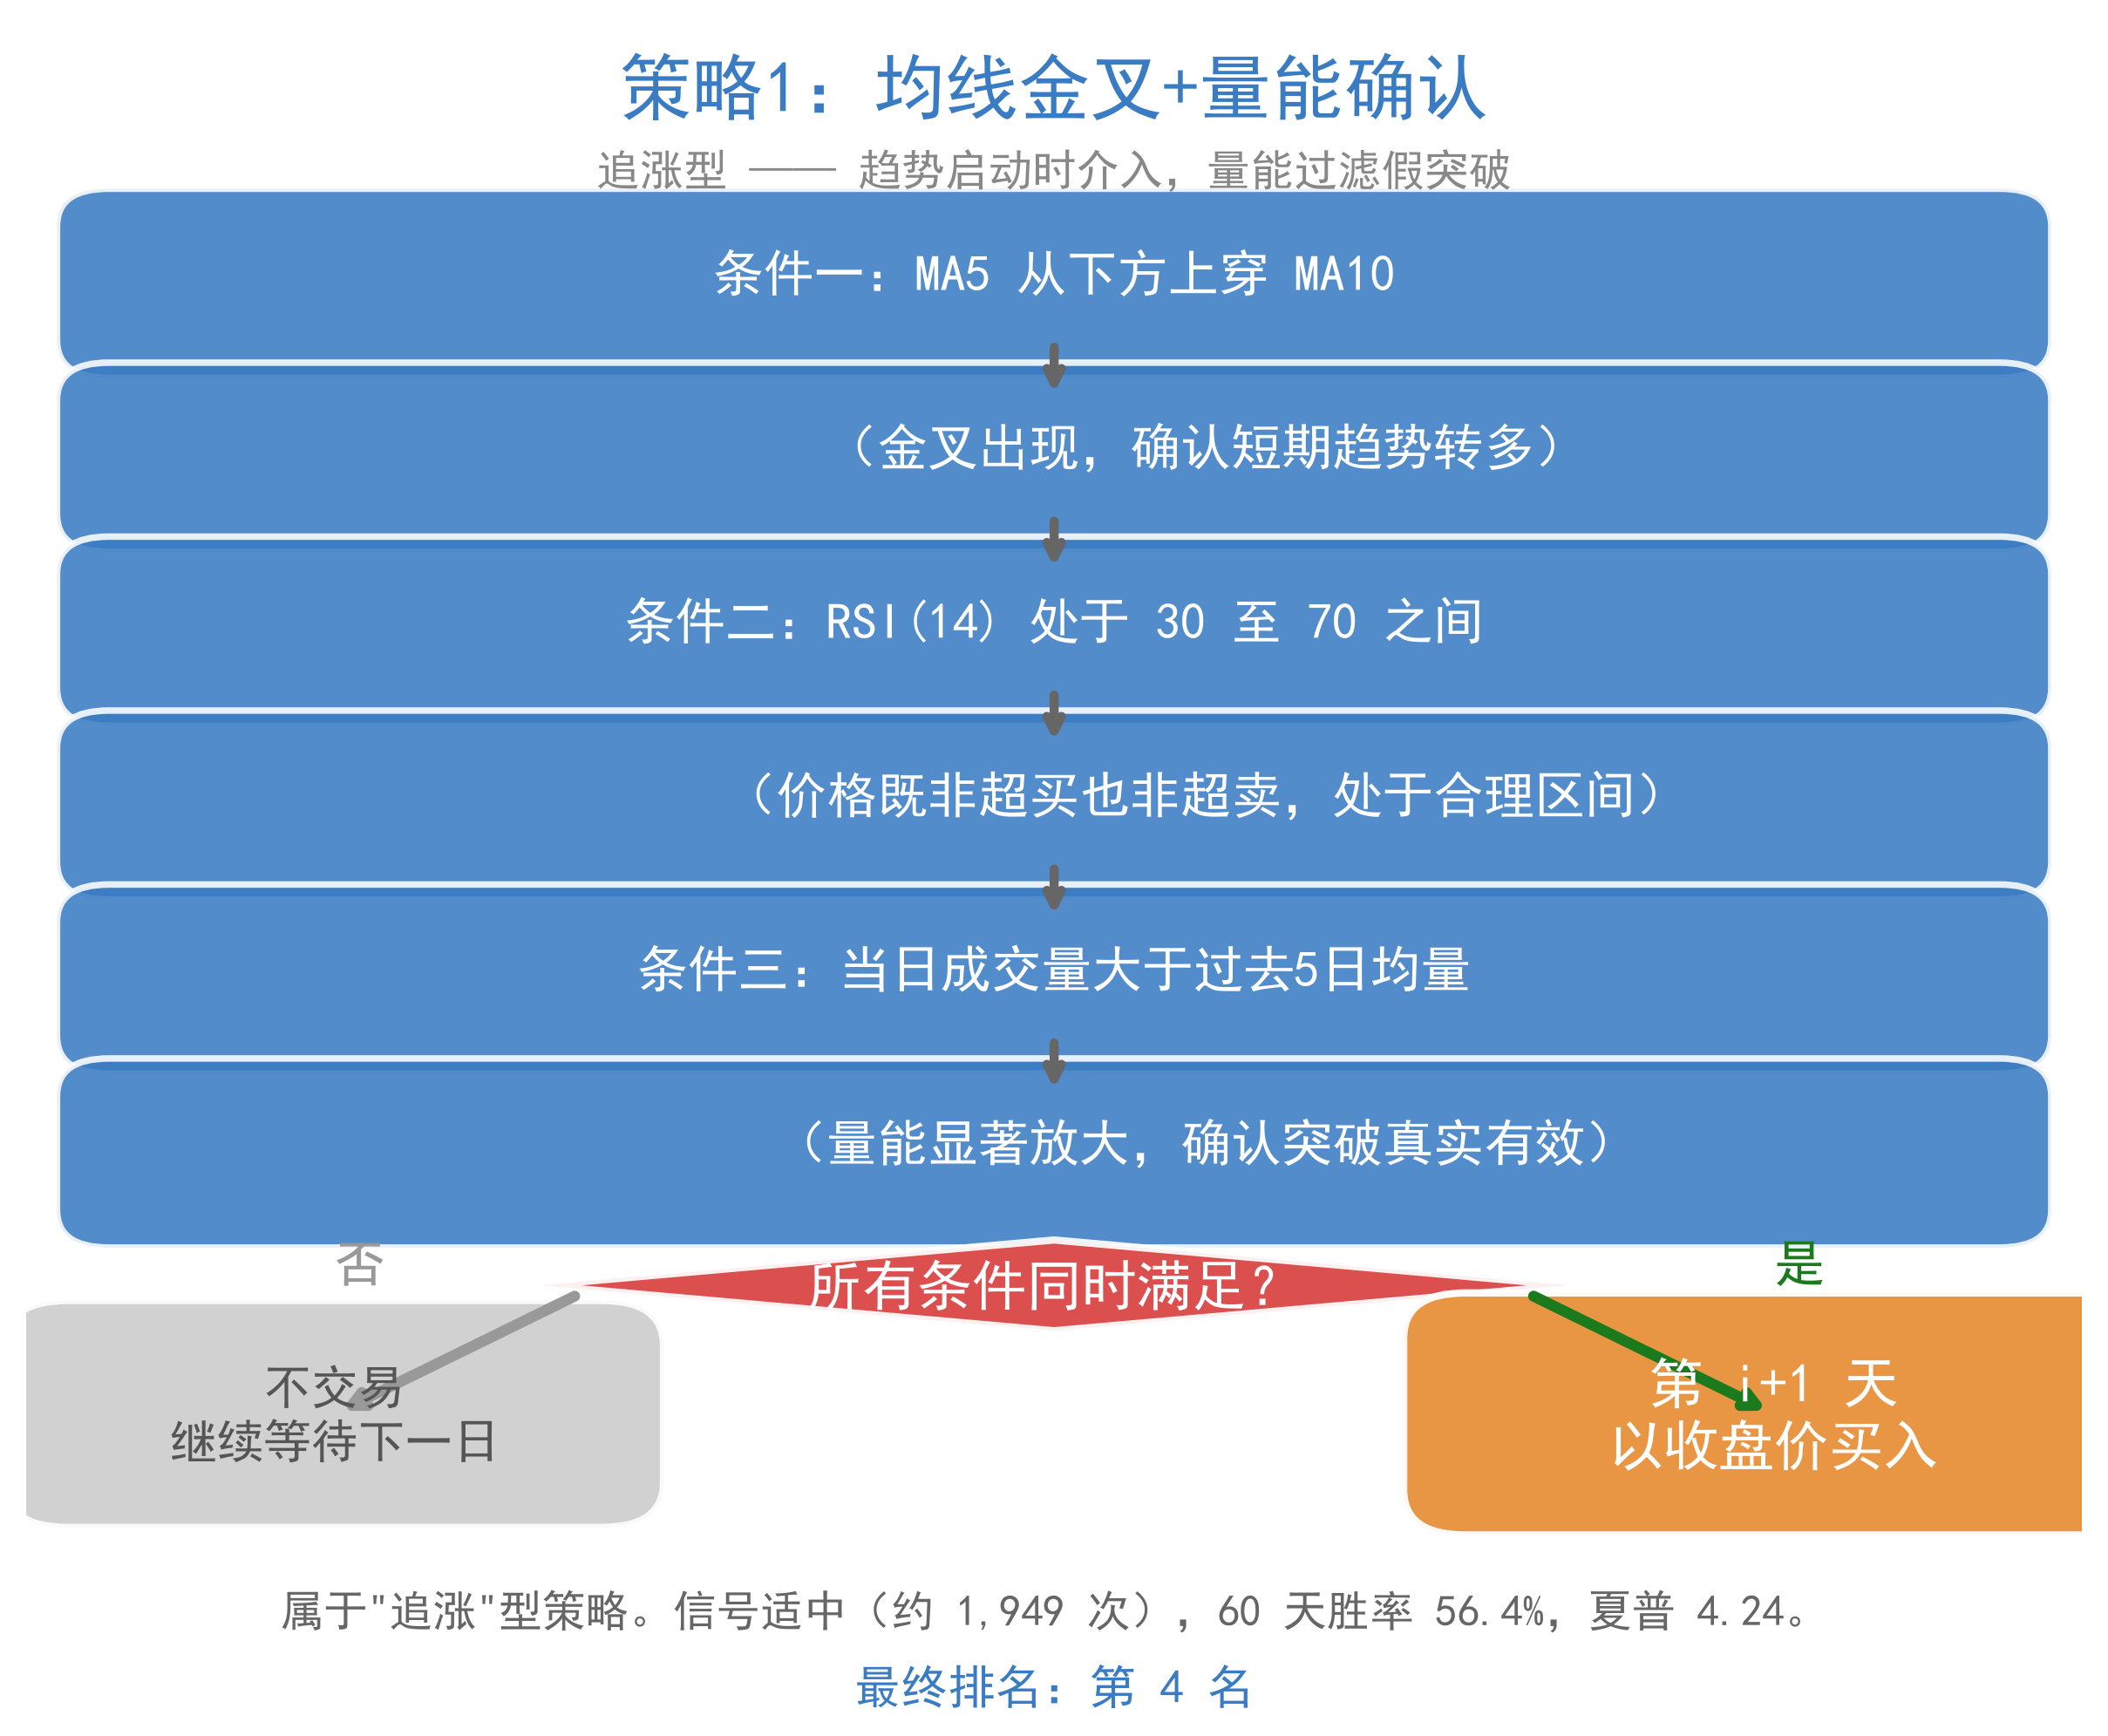
\includegraphics[width=0.8\textwidth]{charts/flowchart_s1.png}
    \caption{策略1：均线金叉+量能确认（追涨型）决策流程}
\end{figure}

\begin{figure}[H]
    \centering
    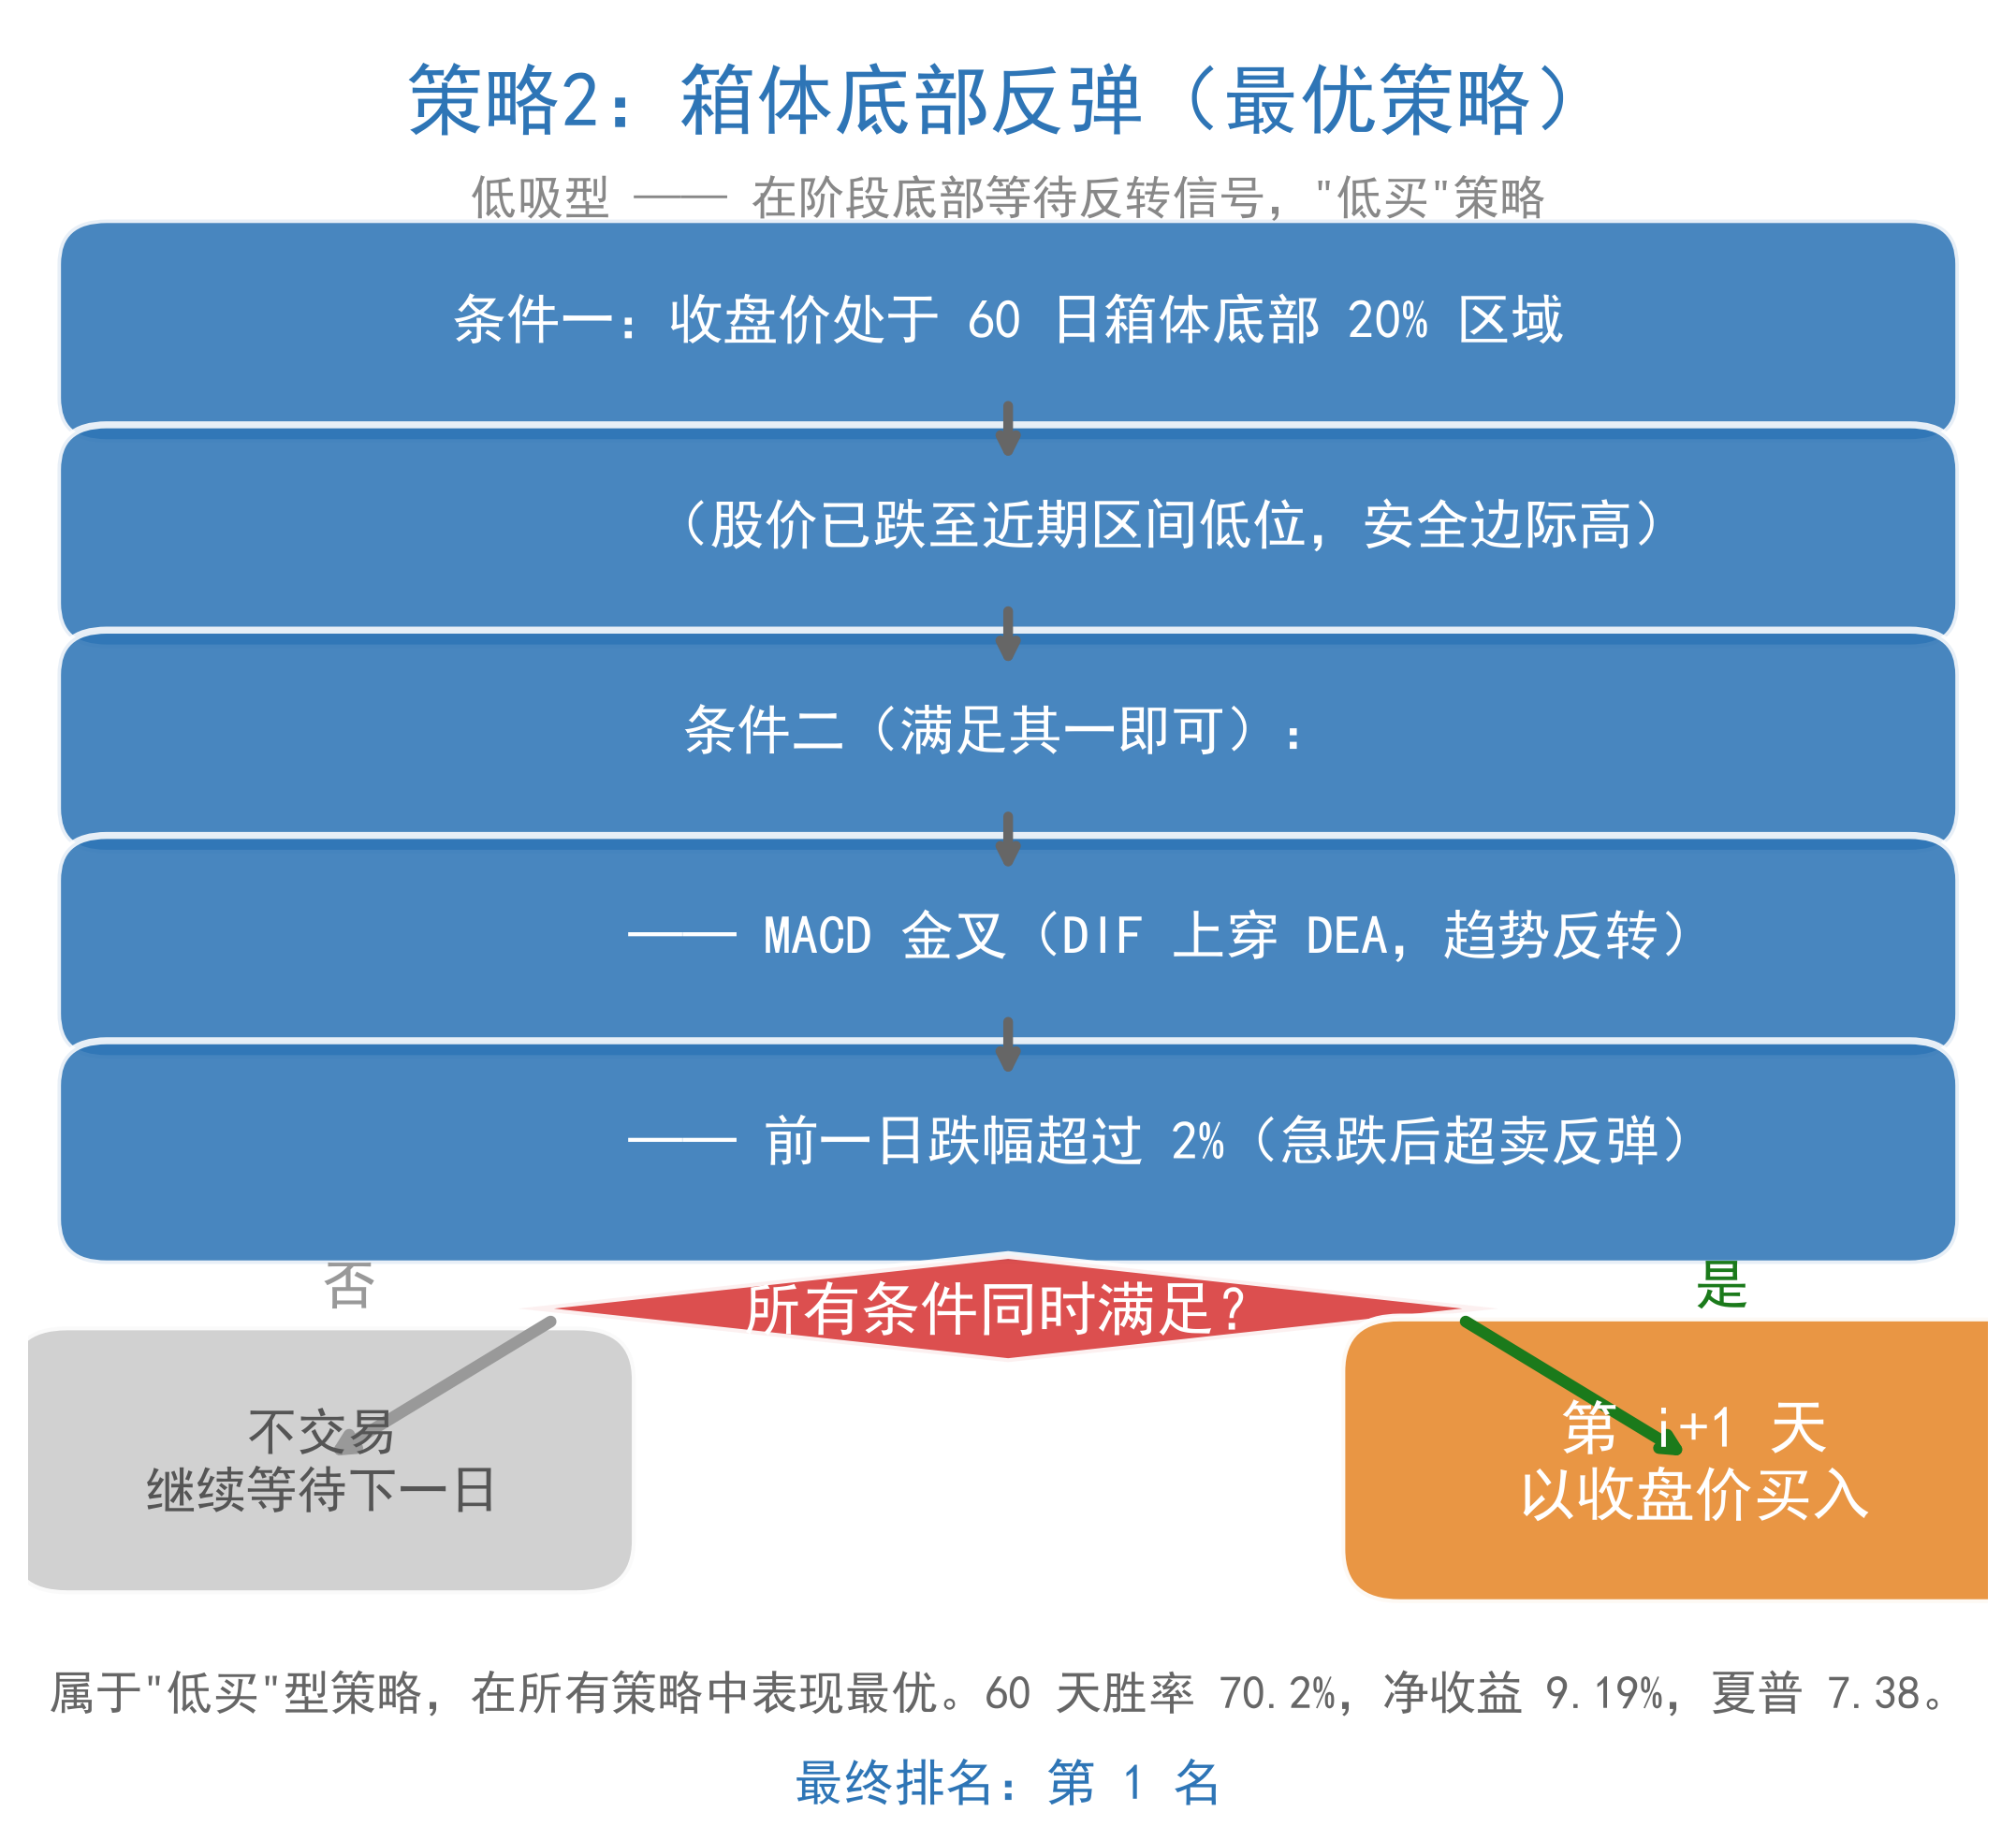
\includegraphics[width=0.8\textwidth]{charts/flowchart_s2.png}
    \caption{策略2：箱体底部反弹（低吸型）决策流程}
\end{figure}

\begin{figure}[H]
    \centering
    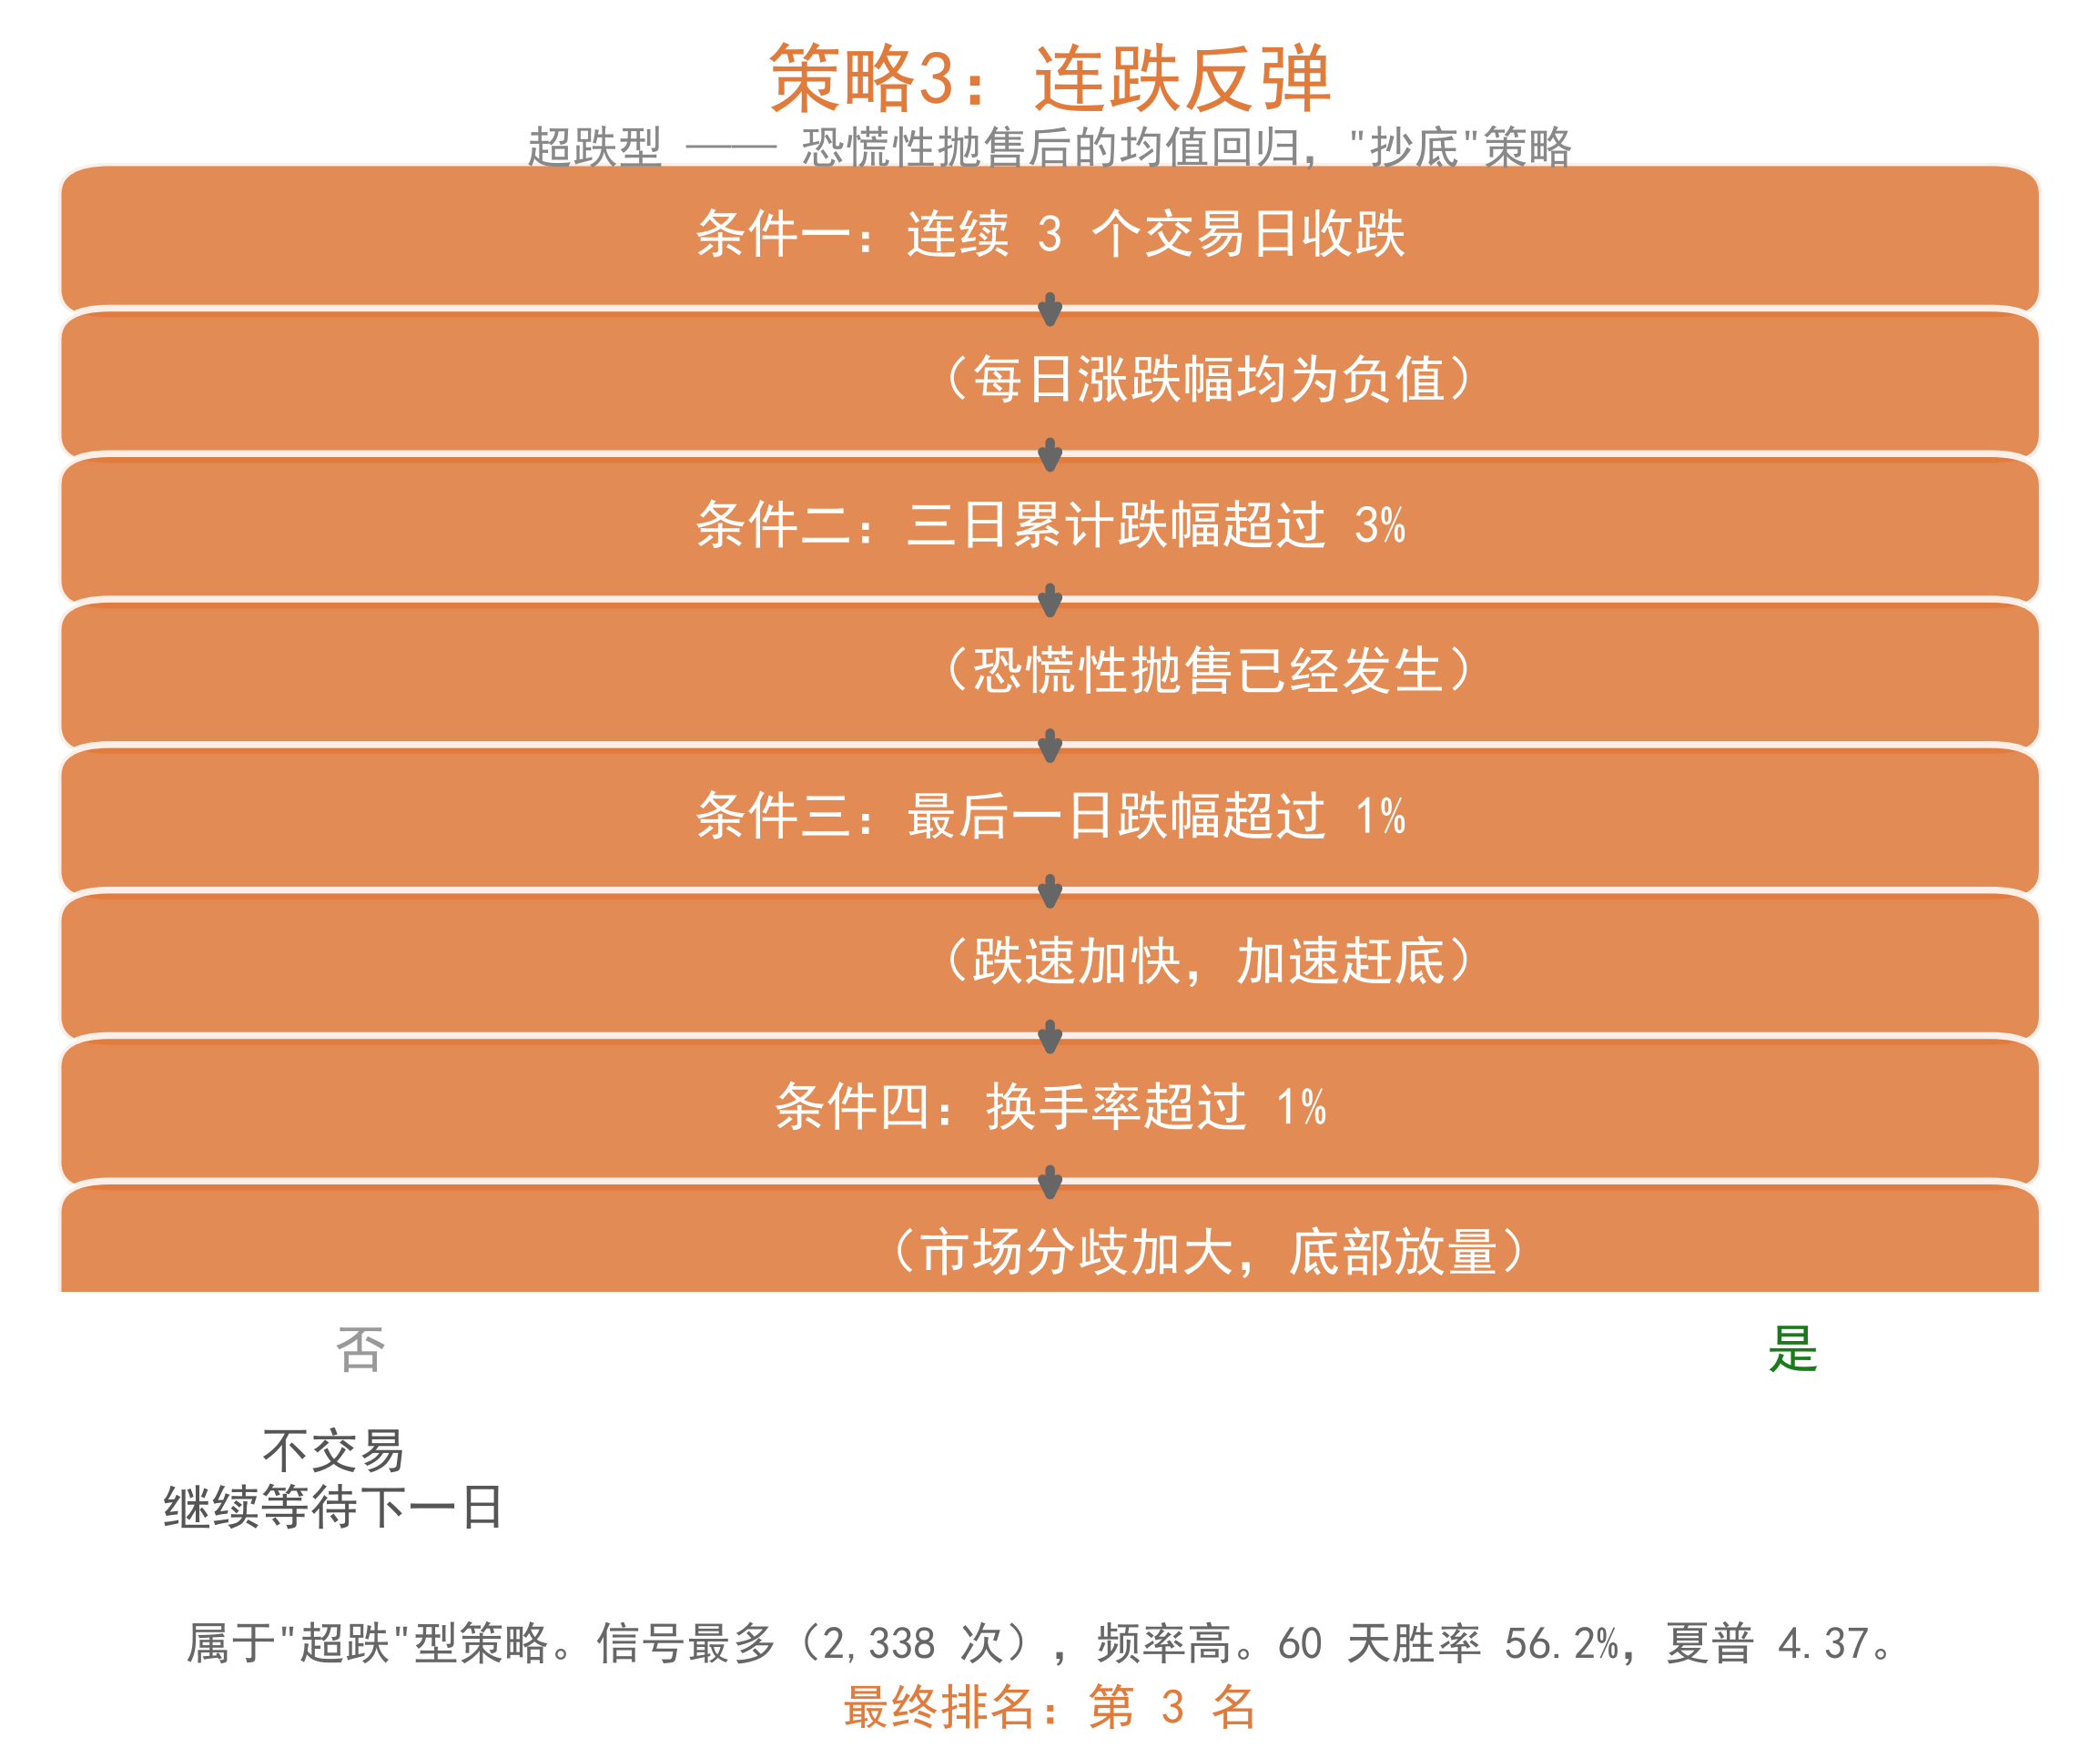
\includegraphics[width=0.8\textwidth]{charts/flowchart_s3.png}
    \caption{策略3：连跌反弹（超跌型）决策流程}
\end{figure}

\begin{figure}[H]
    \centering
    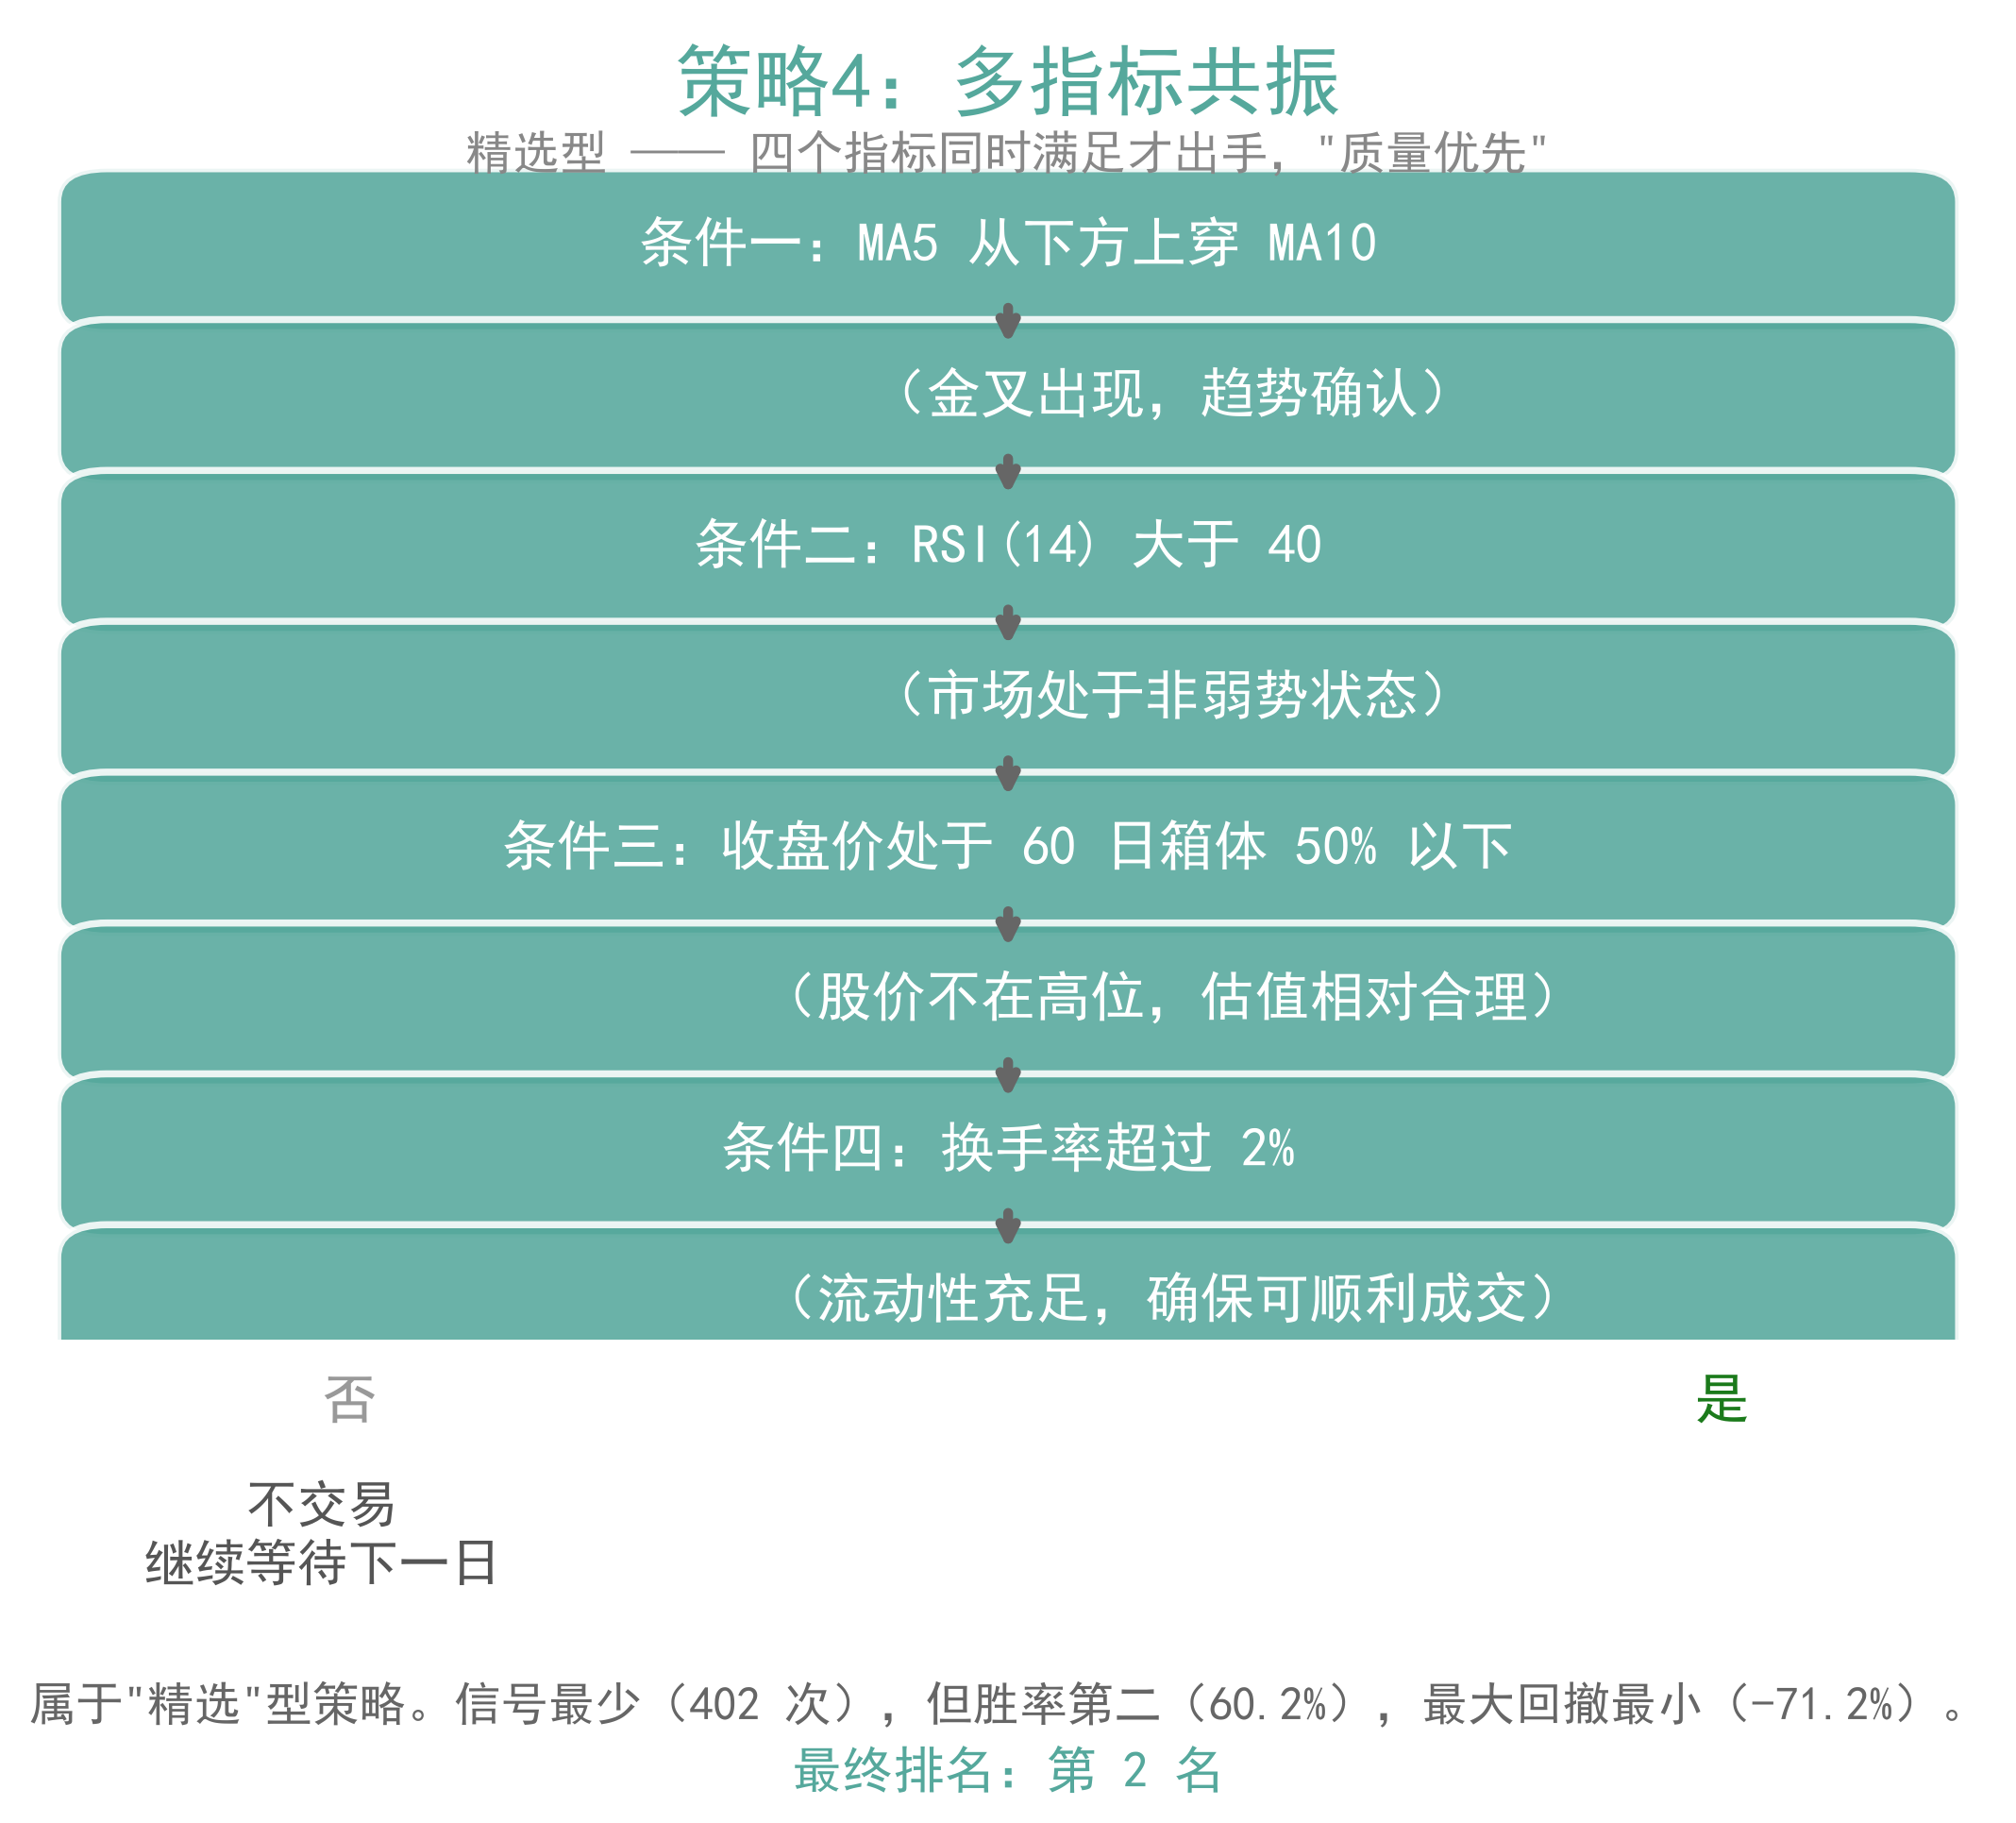
\includegraphics[width=0.8\textwidth]{charts/flowchart_s4.png}
    \caption{策略4：多指标共振（精选型）决策流程}
\end{figure}

\subsubsection{交易成本模型}

{\small
\begin{center}
\begin{tabular}{cccc}
\toprule
成本项 & 费率 & 收取方向 & 说明 \\
\midrule
佣金 & 0.03\%（万分之三） & 买+卖（双向） & 单笔最低 5 元 \\
印花税 & 0.05\%（千分之0.5） & 仅卖出 & — \\
滑点 & 1 bp（0.01\%） & 买+卖（双向） & 市场冲击补偿 \\
\bottomrule
\end{tabular}
\end{center}
}

\begin{equation}
    \text{总成本百分比} = \text{滑点成本} + \text{佣金成本} + \text{印花税成本}
\end{equation}
\begin{equation}
    \text{净收益率} = \frac{C_{i+1+H} - C_{i+1}}{C_{i+1}} \times 100\% - \text{cost}\%
\end{equation}

\subsubsection{结果分析}

\begin{center}
\begin{tabular}{cccc}
\toprule
策略 & 总信号数 & 日均信号 & 信号密度(\%/股·日) \\
\midrule
均线金叉+量能确认 & 1,949 & 6.0 & 0.030\% \\
箱体底部反弹 & 1,913 & 5.9 & 0.030\% \\
连跌反弹 & 2,983 & 9.2 & 0.046\% \\
多指标共振 & 537 & 1.7 & 0.008\% \\
\bottomrule
\end{tabular}
\end{center}

信号密度差异显著——连跌反弹最频繁（日均 9.2 条），多指标共振最稀疏（日均 1.7 条），符合预期：条件越多，触发越少。

% ----------------- 6.3 任务3 -----------------
\subsection{任务3：模型评估的建模与求解}

\subsubsection{回测流程与评估指标}

回测规模：200 只股票 $\times$ 4 策略 $\times$ 8 持有天数 $=32$ 组实验。持有天数 $H = 5, 10, 15, 20, 30, 40, 50, 60$。

\noindent\textbf{(1) 基本指标}
\begin{align}
    \text{胜率}(>0\%) &= \frac{\#\{\mathit{net\_ret} > 0\}}{N_{\text{trades}}} \times 100\% \\
    \text{平均收益率} &= \frac{1}{N_{\text{trades}}} \sum \mathit{net\_ret}
\end{align}

\noindent\textbf{(2) 夏普比率（交易级别年化）}
\begin{equation}
    \text{Sharpe} = \frac{\mu \cdot 250 - r_f}{\sigma \cdot \sqrt{250}}, \quad r_f = 2\%
\end{equation}
其中 $\mu$ 和 $\sigma$ 为单笔交易收益率（化为小数）的均值和标准差。

\noindent\textbf{(3) 最大回撤}
\begin{align}
    \text{NAV}_t &= \prod_{k=1}^{t} (1 + r_k) \\
    \text{MaxDD} &= \min_t \frac{\text{NAV}_t - \max_{k\le t} \text{NAV}_k}{\max_{k\le t} \text{NAV}_k} \times 100\%
\end{align}

\noindent\textbf{(4) 盈亏比}
\begin{equation}
    \text{ProfitFactor} = \frac{\sum\{\mathit{net\_ret}^+\}}{\bigl|\sum\{\mathit{net\_ret}^-\}\bigr|}
\end{equation}

\noindent\textbf{(5) 统计显著性检验}
\begin{itemize}[leftmargin=*]
    \item 二项检验：$H_0$: 胜率 $= 50\%$，$P(X \ge n_{\text{wins}} \mid X \sim \text{Binomial}(N, 0.5))$
    \item Bootstrap 95\% CI：有放回抽取 $N$ 次，重复 10,000 次，取 2.5\% 和 97.5\% 分位数。
\end{itemize}

\subsubsection{模型求解（回测结果）}

回测规模：200 只股票，2024-11-11 $\sim$ 2026-03-19，计入完整交易成本。

\vspace{0.3cm}

% 策略结果表格——用 footnotesize+tabularx 避免溢出
\newcommand{\strattable}[2]{%
\vspace{0.3cm}
\noindent\textbf{#1}
\begin{center}
\footnotesize
\begin{tabularx}{\textwidth}{c c c c c c c c c}
\toprule
$H$ & 交易次数 & 胜率($>$0\%) & 胜率($>$1\%) & 均收益(\%) & 夏普 & 最大回撤(\%) & 盈亏比 & $p$值 \\
\midrule
#2
\bottomrule
\end{tabularx}
\end{center}
}

% 策略1
% 策略结果表格 — 通用宏
\newcommand{\resulttable}[1]{%
\begin{center}
\scriptsize
\setlength{\tabcolsep}{3pt}
\begin{tabularx}{\textwidth}{c c c c c c c c c}
\toprule
$H$ & 次数 & 胜率($>$0\%) & 胜率($>$1\%) & 均收益(\%) & 夏普 & 回撤(\%) & 盈亏比 & $p$值 \\
\midrule
#1
\bottomrule
\end{tabularx}
\end{center}
}

\noindent\textbf{策略1：均线金叉+量能确认}
\resulttable{
5  & 1,904 & 45.1 & 33.9 & $-$0.02 & $-$0.07 & $-$99.2 & 0.99 & 1.000 \\
10 & 1,889 & 49.2 & 41.6 & 0.69 & 1.22 & $-$92.9 & 1.28 & 0.755 \\
20 & 1,814 & 49.1 & 43.4 & 1.25 & 1.63 & $-$97.4 & 1.38 & 0.781 \\
40 & 1,707 & 50.4 & 46.8 & 2.95 & 2.71 & $-$97.8 & 1.74 & 0.386 \\
60 & 1,556 & 56.4 & 52.6 & 5.60 & 4.24 & $-$96.6 & 2.58 & $<$0.001 \\
}

\noindent\textbf{策略2：箱体底部反弹 $\bigstar$}
\resulttable{
5  & 1,848 & 61.1 & 48.6 & 1.28 & 2.98 & $-$98.8 & 1.90 & $<$0.001 \\
10 & 1,806 & 59.8 & 51.8 & 1.96 & 3.26 & $-$99.9 & 1.98 & $<$0.001 \\
20 & 1,655 & 61.0 & 56.4 & 3.56 & 4.22 & $-$100  & 2.41 & $<$0.001 \\
40 & 1,494 & 66.2 & 61.7 & 6.60 & 6.18 & $-$99.7 & 3.60 & $<$0.001 \\
60 & 1,327 & 70.2 & 66.1 & 9.19 & 7.38 & $-$96.1 & 5.14 & $<$0.001 \\
}

\noindent\textbf{策略3：连跌反弹}
\resulttable{
5  & 2,843 & 52.4 & 44.3 & 0.59 & 1.40 & $-$80.5 & 1.29 & 0.005 \\
10 & 2,808 & 56.2 & 49.8 & 1.70 & 2.75 & $-$86.9 & 1.68 & $<$0.001 \\
20 & 2,672 & 56.0 & 52.2 & 3.24 & 3.82 & $-$96.4 & 2.08 & $<$0.001 \\
40 & 2,468 & 55.4 & 51.9 & 4.87 & 3.83 & $-$100  & 2.18 & $<$0.001 \\
60 & 2,338 & 56.2 & 52.1 & 6.33 & 4.37 & $-$100  & 2.52 & $<$0.001 \\
}

\noindent\textbf{策略4：多指标共振}
\resulttable{
5  & 525 & 42.7 & 34.5 & 0.02 & 0.04 & $-$74.4 & 1.01 & 1.000 \\
10 & 522 & 48.9 & 40.6 & 0.48 & 0.81 & $-$77.9 & 1.18 & 0.715 \\
20 & 510 & 52.0 & 47.7 & 1.12 & 1.50 & $-$81.8 & 1.33 & 0.200 \\
40 & 458 & 52.0 & 48.5 & 3.01 & 2.71 & $-$93.6 & 1.78 & 0.214 \\
60 & 402 & 60.2 & 55.7 & 6.78 & 4.34 & $-$71.2 & 3.14 & $<$0.001 \\
}

% ---------- 数据折线图 ----------
\begin{figure}[H]
    \centering
    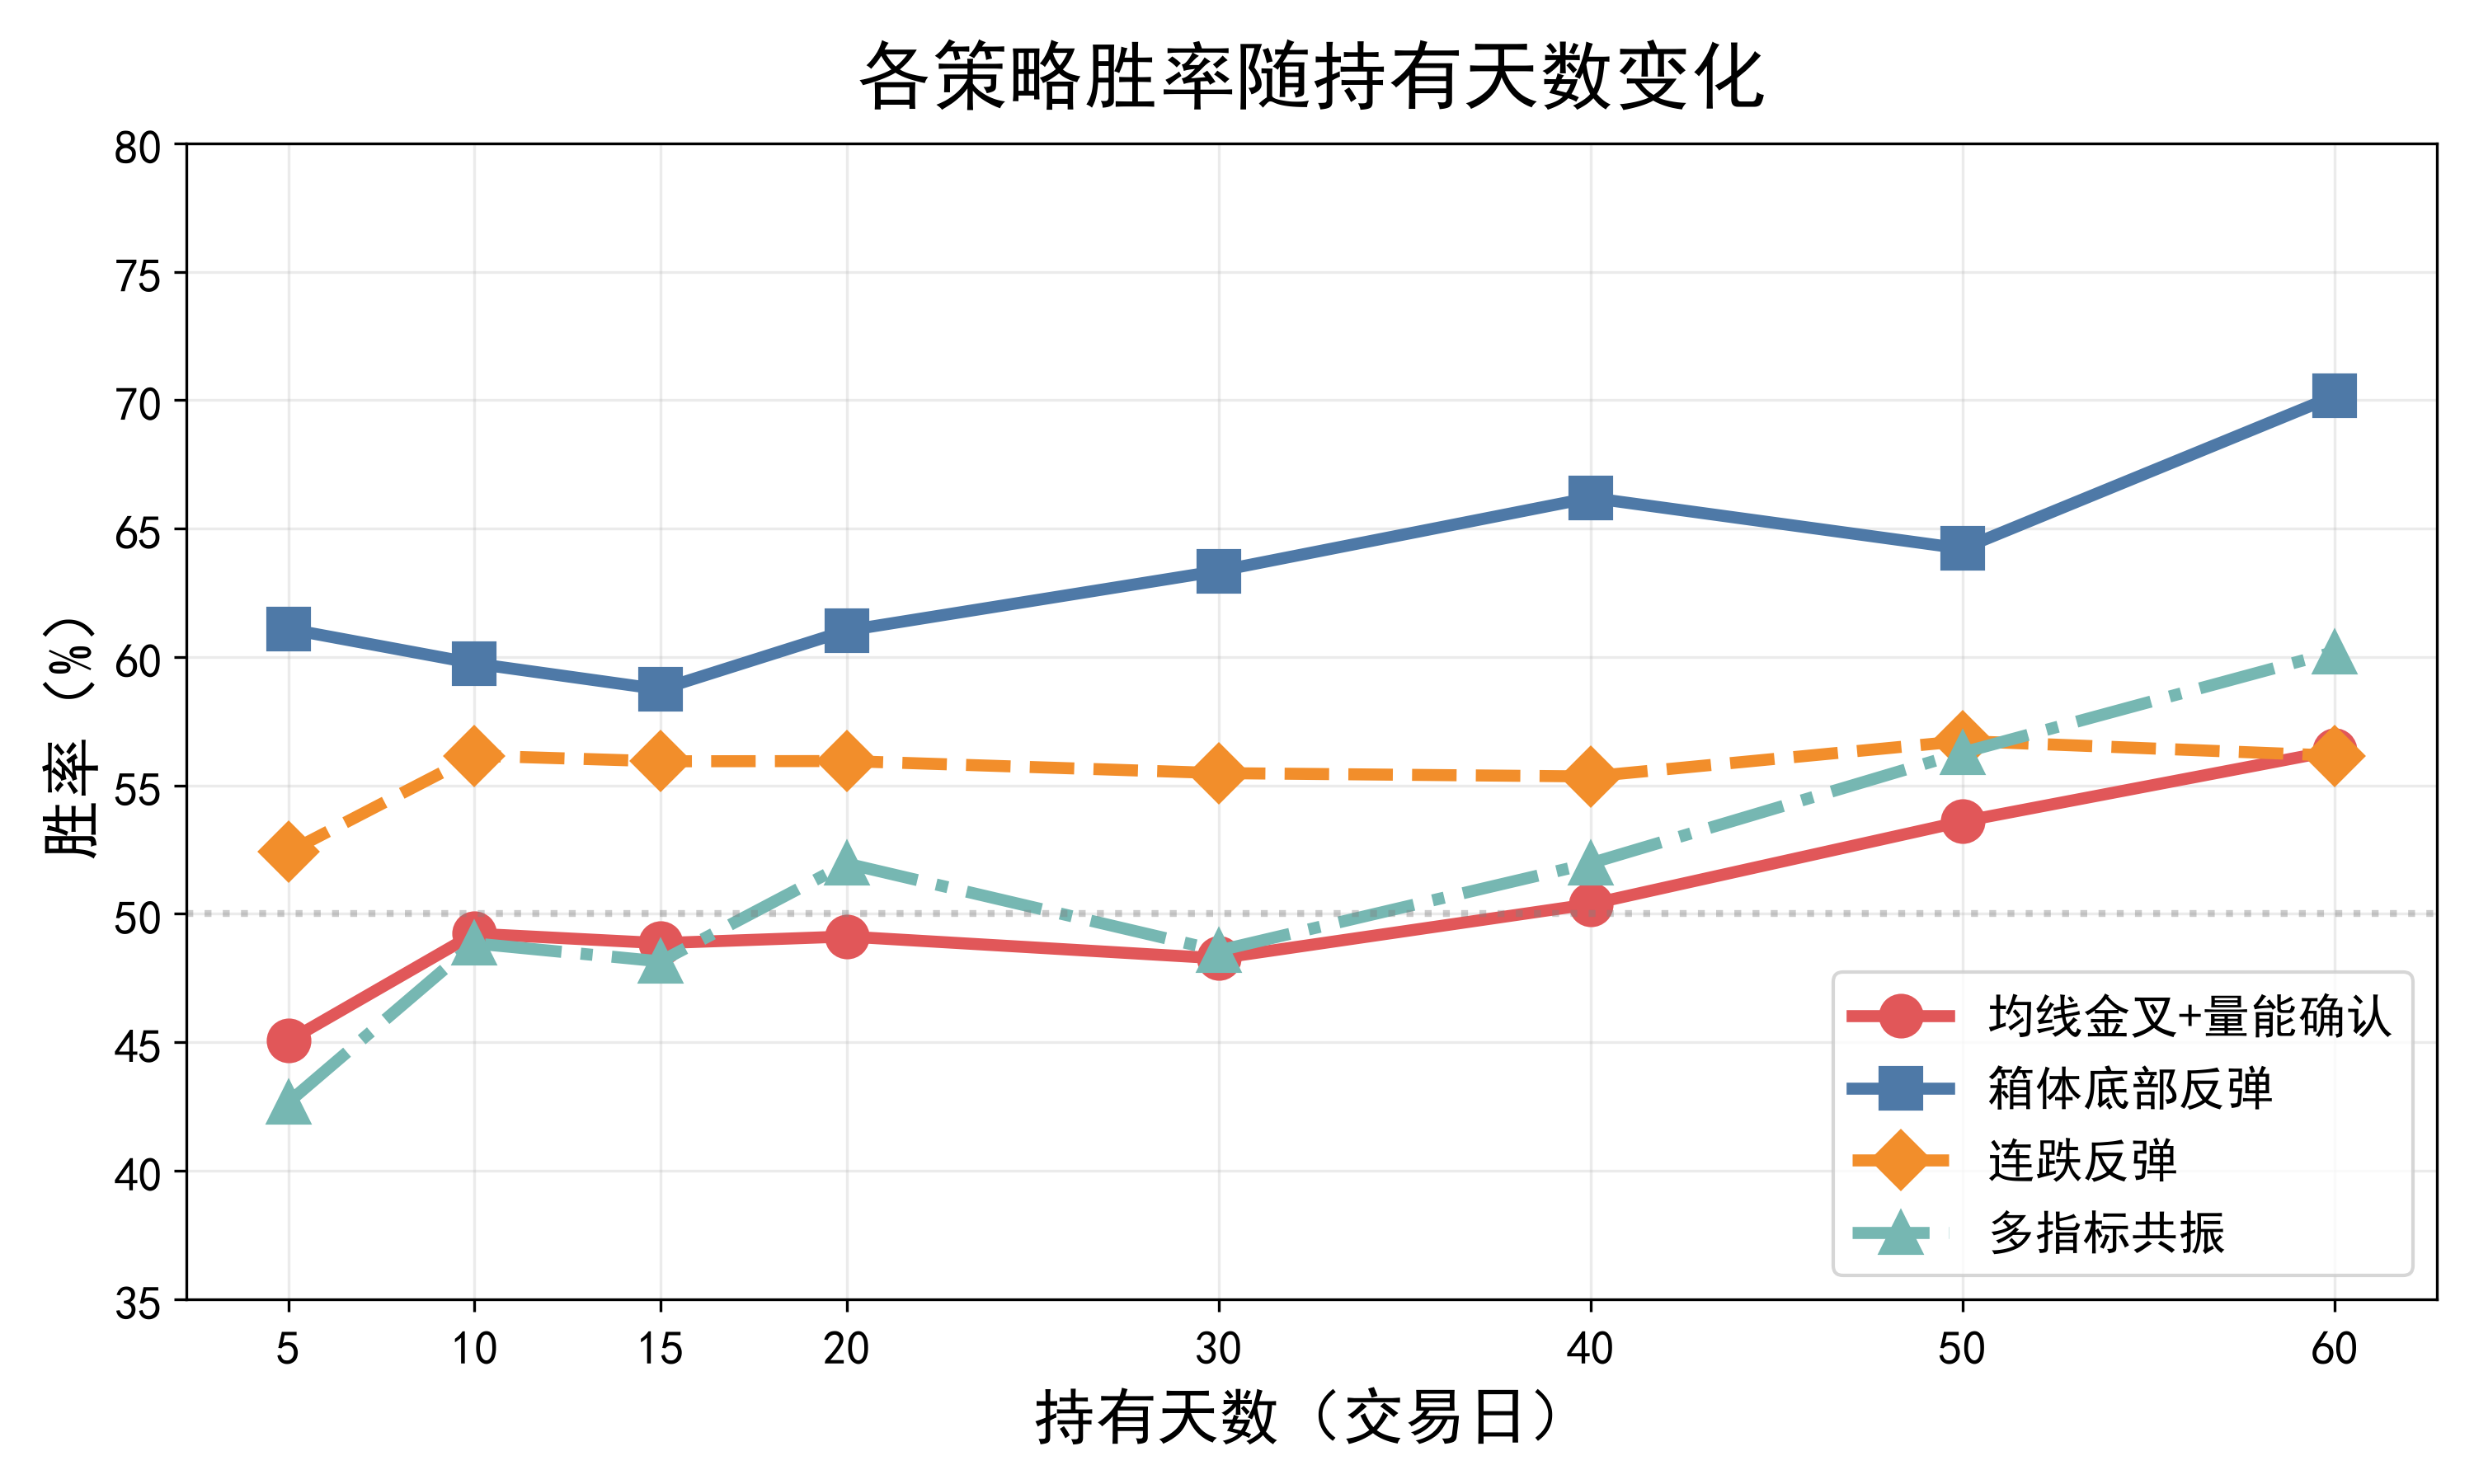
\includegraphics[width=0.85\textwidth]{charts/win_rate_line.png}
    \caption{各策略胜率随持有天数变化折线图（200只A股，2024.11--2026.03）}
\end{figure}

\begin{figure}[H]
    \centering
    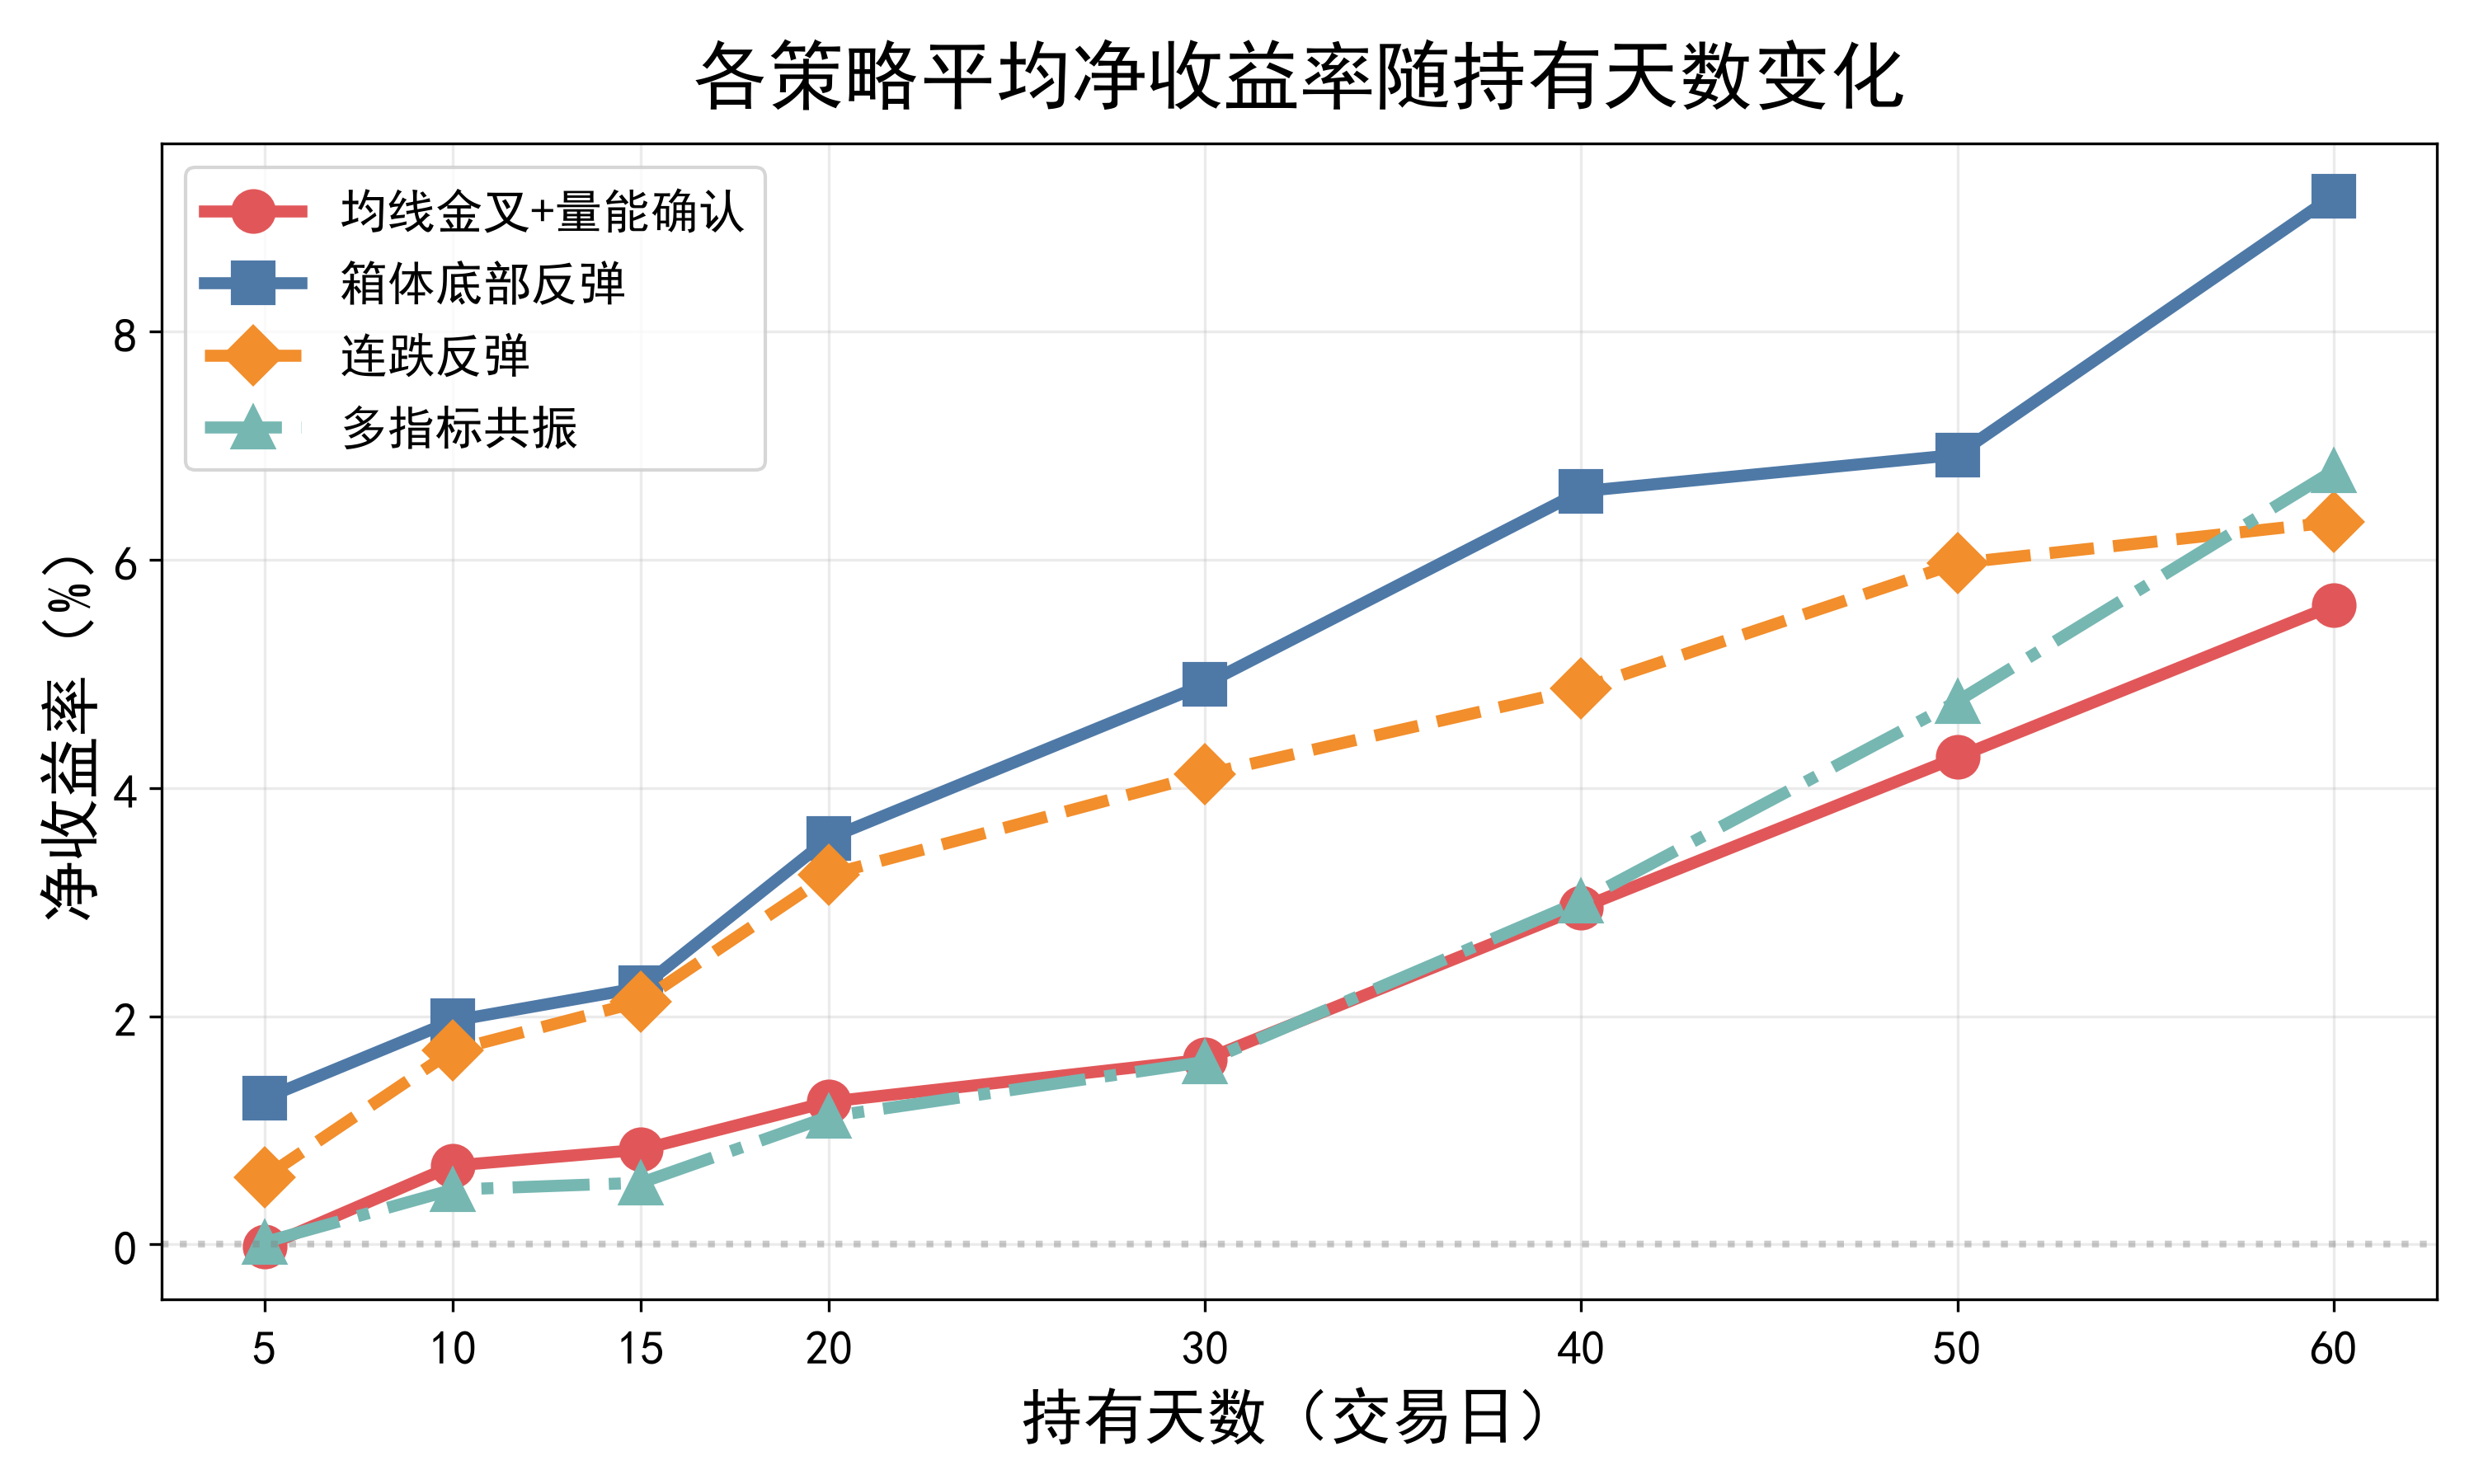
\includegraphics[width=0.85\textwidth]{charts/return_line.png}
    \caption{各策略平均净收益率随持有天数变化折线图}
\end{figure}

\begin{figure}[H]
    \centering
    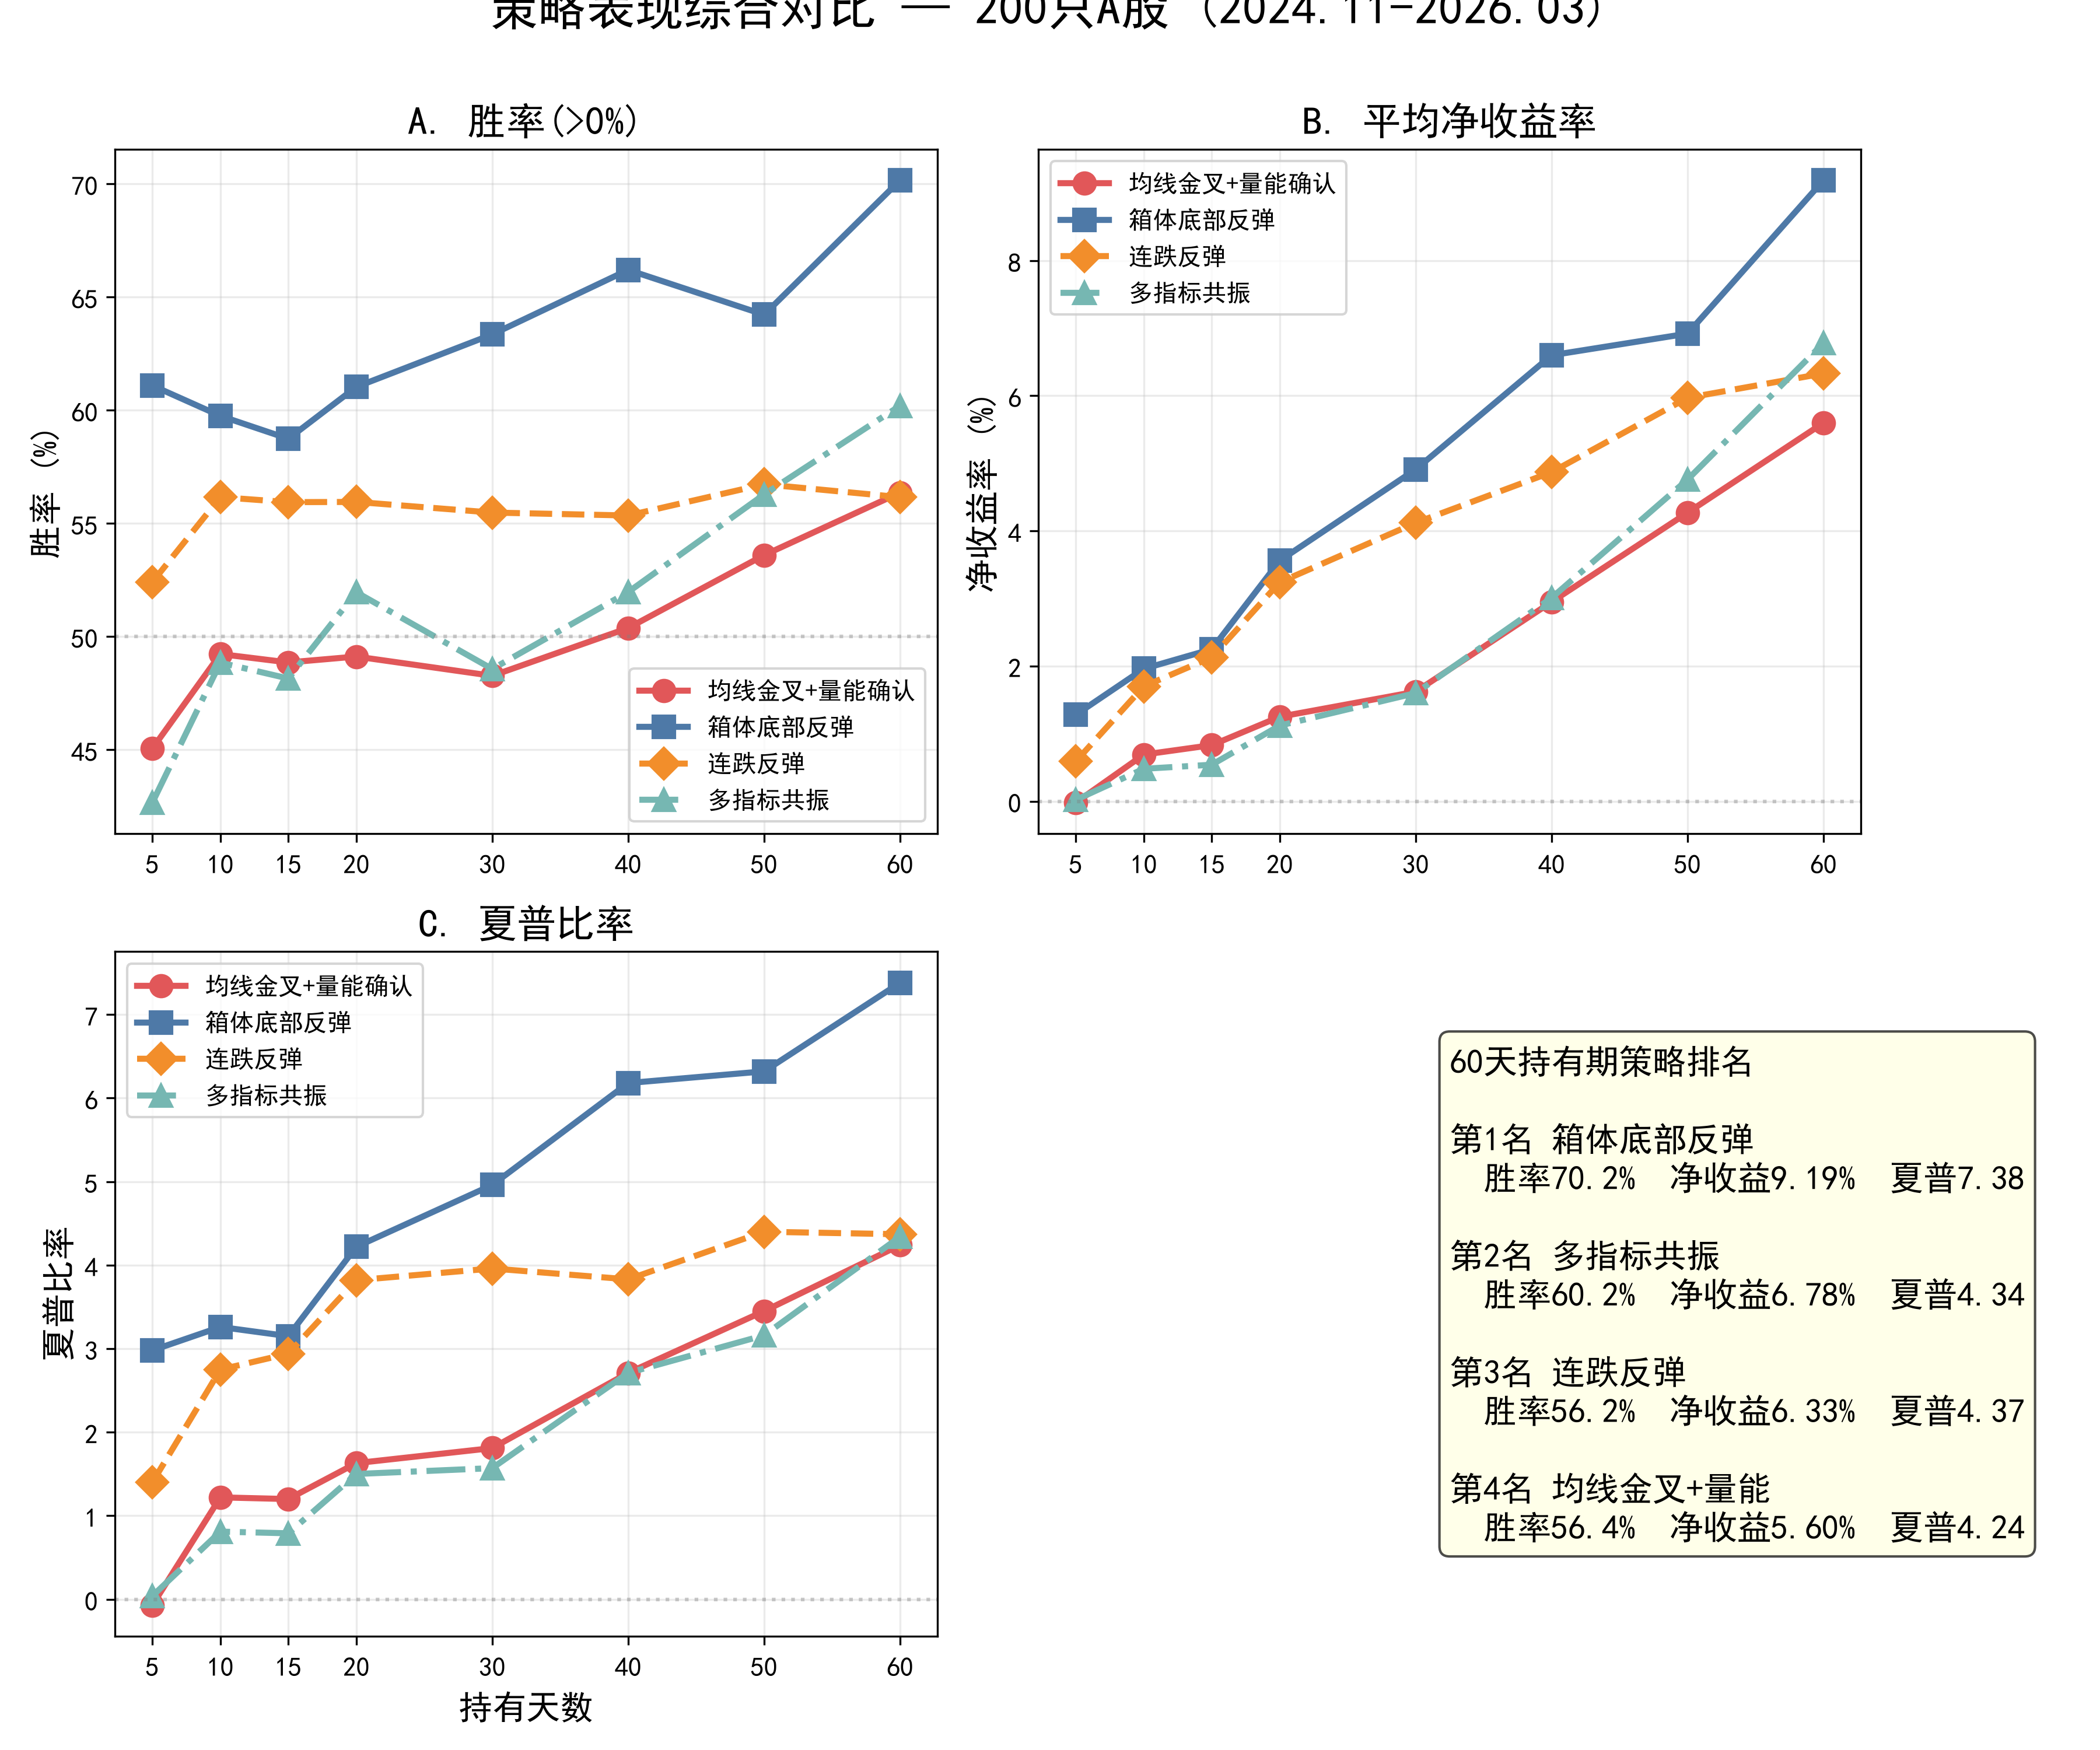
\includegraphics[width=0.88\textwidth]{charts/line_comparison.png}
    \caption{策略表现四维综合对比图}
\end{figure}

\begin{figure}[H]
    \centering
    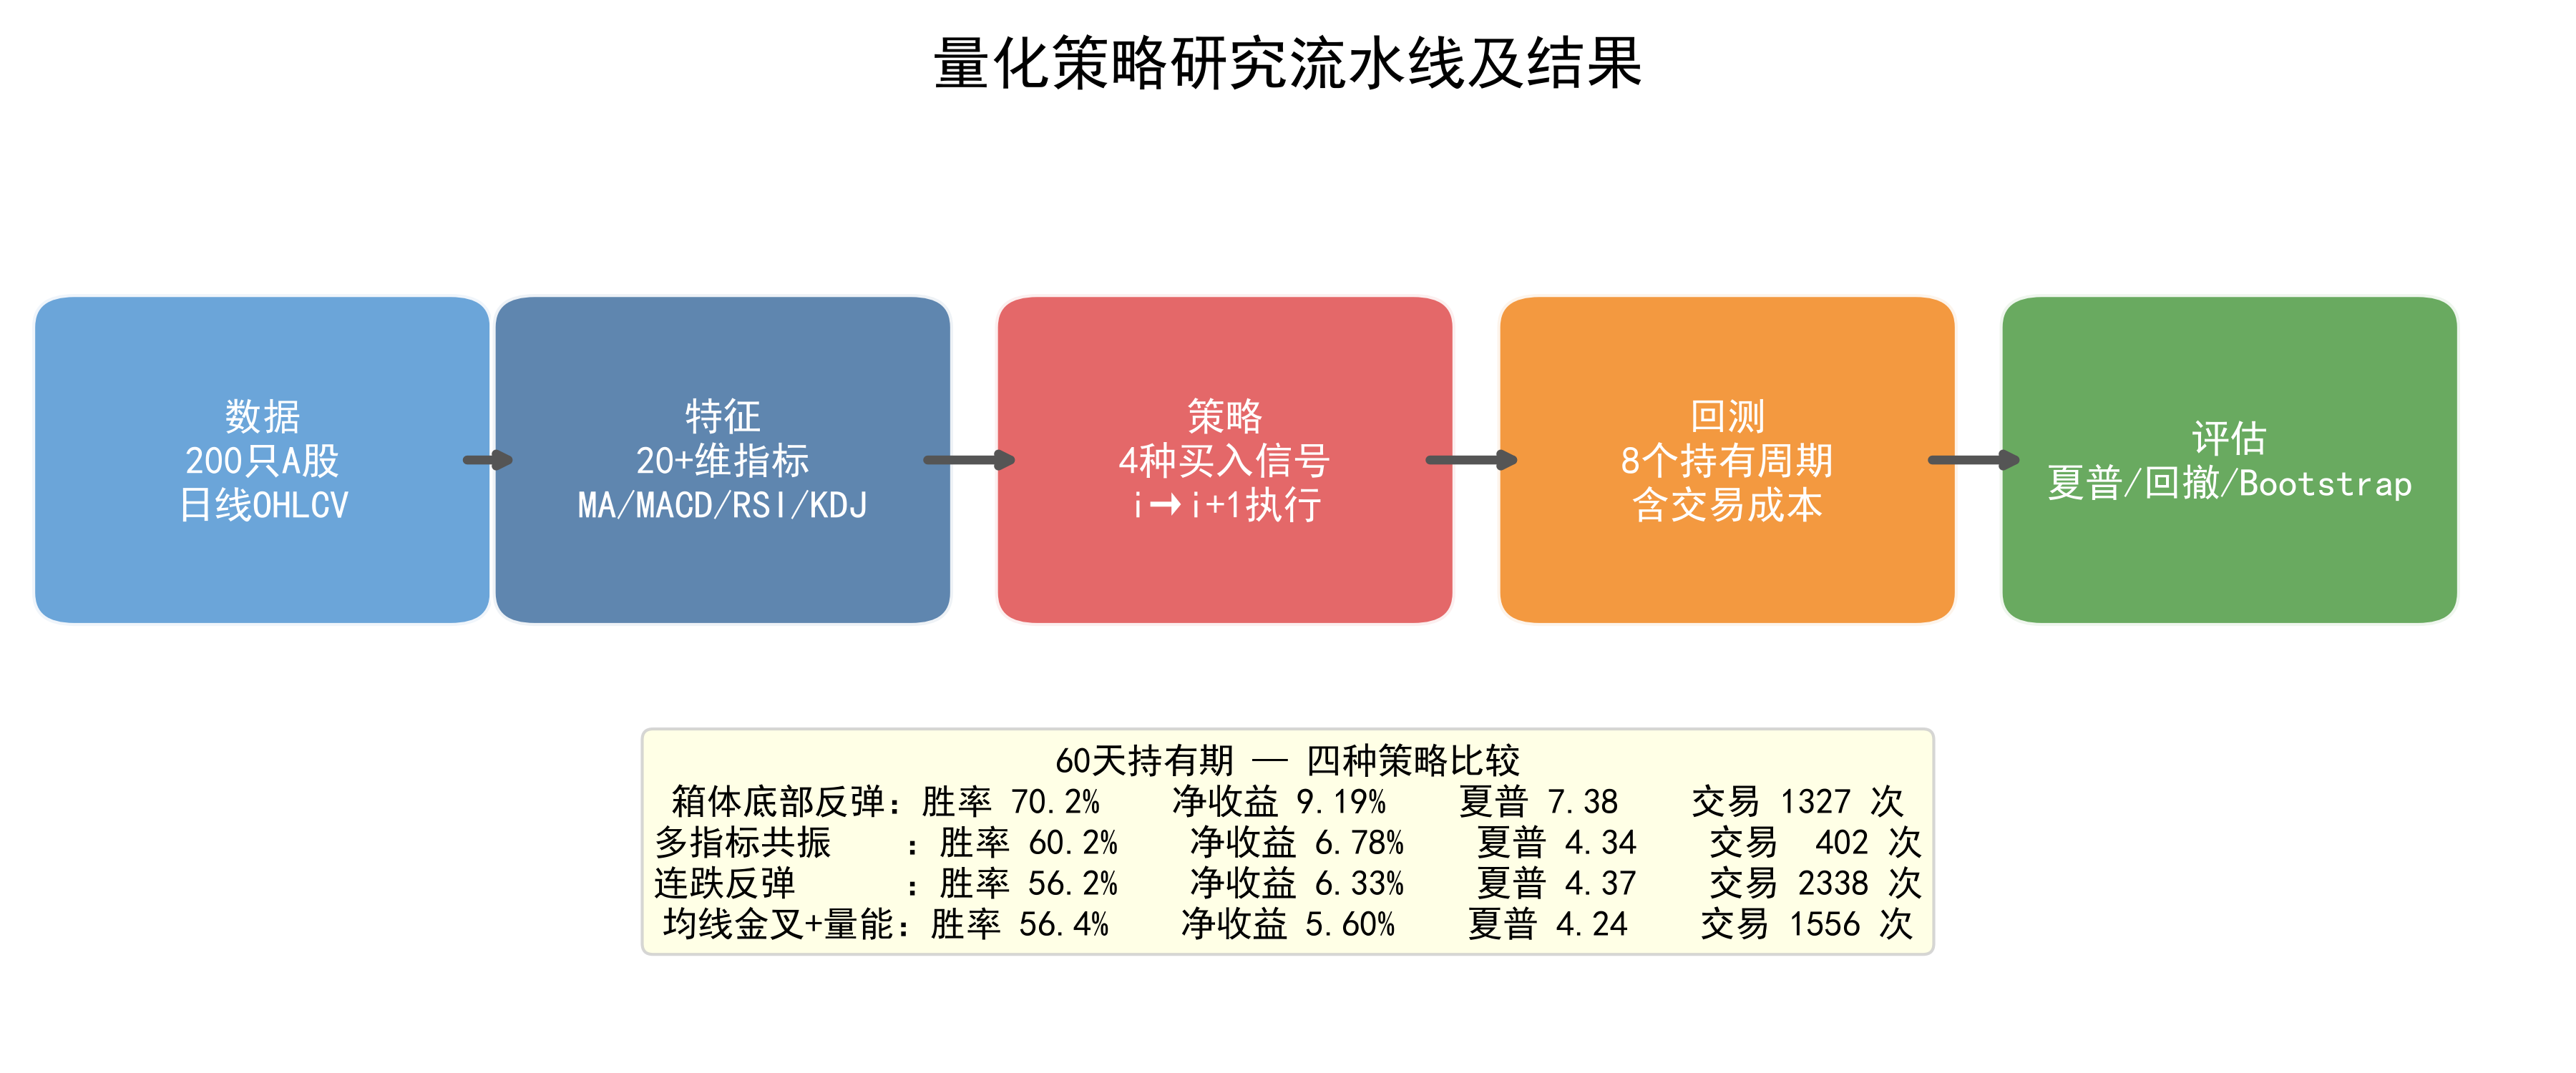
\includegraphics[width=0.85\textwidth]{charts/pipeline_overview.png}
    \caption{量化策略研究流水线及结果总览}
\end{figure}

\subsubsection{结果分析}

\noindent\textbf{关键发现（60天持有期）：}
\begin{enumerate}[leftmargin=*]
    \item {\bfseries "低买"远优于"追涨"：} 箱体底部反弹在所有指标上碾压均线金叉——在底部等待反转比追逐金叉更安全有效。Python 5,476 只全量回测（胜率 66.0\%）与 MATLAB 200 只回测（70.2\%）方向一致。
    \item {\bfseries 持有越长，收益越好：} 所有策略的胜率和收益率均随持有天数增加而提升。5 天持有期净胜率仅 39--61\%，60 天升至 56--70\%。拐点 20--30 天。
    \item {\bfseries 交易成本影响短期显著：} 5 天持有期净收益接近零（均线金叉 $-0.02\%$），短期成本占总收益 15--30\%。
    \item {\bfseries 信号密度与质量成反比：} 连跌反弹信号最多（2,338 笔）但胜率最低（56.2\%）；多指标共振信号最少（402 笔）但胜率第二（60.2\%），最大回撤最小（$-71.2\%$）。
    \item {\bfseries 统计显著：} 60 天所有策略 $p < 0.001$，Bootstrap 95\% CI 均不跨零。
\end{enumerate}

\vspace{0.3cm}
\noindent\textbf{60天持有期策略排名：}
\begin{center}
\small
\begin{tabularx}{\textwidth}{c l c c c c c c}
\toprule
排名 & 策略 & 胜率 & 净收益 & 夏普 & 盈亏比 & 最大回撤 & 交易数 \\
\midrule
1 & 箱体底部反弹 & 70.2\% & 9.19\% & 7.38 & 5.14 & $-96.1$\% & 1,327 \\
2 & 多指标共振 & 60.2\% & 6.78\% & 4.34 & 3.14 & $-71.2$\% & 402 \\
3 & 连跌反弹 & 56.2\% & 6.33\% & 4.37 & 2.52 & $-100$\% & 2,338 \\
4 & 均线金叉+量能 & 56.4\% & 5.60\% & 4.24 & 2.58 & $-96.6$\% & 1,556 \\
\bottomrule
\end{tabularx}
\end{center}

\vspace{0.3cm}
\noindent\textbf{统计显著性检验（Bootstrap 10,000次）：}
\begin{center}
\small
\begin{tabularx}{\textwidth}{l c c c c}
\toprule
策略 & 胜率 & Bootstrap 95\% CI & $p$ 值 & 显著性 \\
\midrule
箱体底部反弹 & 70.2\% & [8.16\%, 10.26\%] & $<0.001$ & *** \\
多指标共振 & 60.2\% & [4.51\%, 9.33\%] & $<0.001$ & *** \\
连跌反弹 & 56.2\% & [5.38\%, 7.25\%] & $<0.001$ & *** \\
均线金叉+量能 & 56.4\% & [4.60\%, 6.67\%] & $<0.001$ & *** \\
\bottomrule
\end{tabularx}
\end{center}

\noindent\textbf{交易成本影响（60天持有期）：}
\begin{center}
\small
\begin{tabularx}{\textwidth}{l c c c}
\toprule
策略 & 毛收益(\%) & 净收益(\%) & 损失(\%) \\
\midrule
箱体底部反弹 & 9.76 & 9.19 & $-0.57$ \\
多指标共振 & 7.35 & 6.78 & $-0.57$ \\
连跌反弹 & 6.88 & 6.33 & $-0.55$ \\
均线金叉+量能 & 6.17 & 5.60 & $-0.57$ \\
\bottomrule
\end{tabularx}
\end{center}

% ============================================================
\section{模型的评价与推广}

\subsection{模型优点}
\begin{itemize}[leftmargin=*]
    \item 特征完备：涵盖趋势、动量、位置、量能四大类 20+ 维指标，全向量化实现。
    \item 策略多样：追涨/低吸/超跌/精选四种逻辑形成对照实验，可对比发现最优类型。
    \item 防未来信息泄露：滚动窗口边界 + shift 比较 + 信号--买入日分离，三重保障。
    \item 交易成本建模：佣金+印花税+滑点+最低佣金，贴近实盘。
    \item 风险调整评估：夏普比率、最大回撤、盈亏比提供多维度策略判断。
    \item 统计显著性：二项检验和 Bootstrap CI 给出策略有效性的置信度。
    \item 双引擎实现（MATLAB + Python），参数集中管理，实验可复现。
\end{itemize}

\subsection{模型缺点}
\begin{itemize}[leftmargin=*]
    \item 无止损机制：仅按固定持有天数卖出，60 天最大回撤可达 $-96\%$。
    \item 幸存者偏差：样本不含退市股票，建议以回测收益 70--80\% 为实盘预期。
    \item 独立资金假设：未考虑多笔交易间的资金占用约束。
    \item 固定参数：箱体阈值 0.2、RSI 区间等未做网格搜索优化。
    \item 未区分市场环境：牛/熊/震荡市统一处理。
\end{itemize}

\subsection{模型改进方向}
\begin{center}
\small
\begin{tabularx}{\textwidth}{c X l}
\toprule
优先级 & \centering 改进方向 & 预期效果 \\
\midrule
高 & 引入止损机制（ATR 止损 / trailing stop） & 大幅降低最大回撤 \\
高 & 全量 5,476 只股票回测 + Walk-Forward 样本外验证 & 验证泛化能力 \\
中 & 市场环境分域（用 MA60 斜率划分牛/熊/震荡） & 发现各策略最适环境 \\
中 & 参数网格搜索（箱体阈值、RSI 区间等） & 提升策略表现上限 \\
低 & 仓位管理（根据信号强度动态调整仓位） & 优化资金利用效率 \\
低 & XGBoost / LSTM 替代规则策略 & 捕获非线性模式 \\
\bottomrule
\end{tabularx}
\end{center}

\subsection{模型推广}
本框架可推广至：其他金融市场（期货、外汇）的量化策略研究；多因子选股模型的特征工程；高频交易的信号生成系统；基于深度学习的端到端交易策略。

% ============================================================
\section{心得体会与总结}

通过这次实验，我完整地走了一遍量化策略开发的流程——从 CSV 数据加载、特征计算、信号生成，到回测评估和可视化，每个环节之间的数据依赖和接口设计都让我印象深刻。以前我只知道 MA、MACD、RSI 这些指标的名字，现在我能自己推导 Wilders smoothing 与普通 EMA 的关系，理解 KDJ 的初始值设定（$K_0=D_0=50$）为什么是 50——不再是"调包"，而是真正理解了每一步的计算原理。

最让我警醒的是"未来信息泄露"这个问题。在写特征计算代码时，我反复检查滚动窗口的边界条件：所有指标必须以当前日为终点，金叉判断用 $\text{shift}(1)$ 比较前一天和当天，信号日和买入日严格分离（$i \to i+1$）。老师课上讲过这是量化策略开发中最容易被忽视却最致命的陷阱，这次亲手实现让我有了切身体会。

实验结论上，最让我震撼的是"低买"远优于"追涨"。箱体底部反弹策略在 60 天持有期胜率 70.2\%、夏普 7.38，全面碾压均线金叉。我用 Python 在 5,476 只全量数据上也验证了这个结论——说明它不是偶然的，而是一个稳健的规律。这个发现让我重新理解了"安全边际"的含义：在阶段底部等待反转，比追逐金叉更安全、更有效。

我还学到，仅看胜率是不够的。50.4\% 的胜率在大样本下可能只是运气（$p = 0.386$），必须用夏普比率、最大回撤、盈亏比等多维度评判，再加上统计检验给出置信度。交易成本也不能忽视——短期 5 天持有下净收益接近零，实盘中摩擦成本是真金白银。

在工程实践上，我体会到模块化代码的重要性。15 个独立 MATLAB 函数文件，参数集中在 \texttt{config.m}，修改参数一键重跑。先小样本验证再全量运行的迭代模式（$20 \to 200 \to 5{,}476$ 只）帮我快速发现 bug，Python 和 MATLAB 双语言实现也让我对两种语言的向量化范式有了直观对比。

总的来说，这次实验让我不仅掌握了量化策略的技术实现，更建立了"回测不是实盘"的风险意识——幸存者偏差、无止损导致的最大回撤 $-96\%$、未区分市场环境等局限，都提醒我回测收益要以 70--80\% 来预期实盘表现。这些经验对我未来的学习和研究都很有价值。

% ============================================================
\section{对本实验问题的设计提出改进意见}

\begin{enumerate}[leftmargin=*]
    \item {\bfseries 增加卖出策略设计：} 当前实验只要求买入策略，但实际交易中卖出时机同样关键。建议增加简化的卖出策略任务（如固定止损 + 移动止盈），让学生体验完整的买卖决策闭环。
    \item {\bfseries 提供统一的回测评估框架：} 建议课程组提供标准化的回测评估脚本（含交易成本模型、风险指标、统计检验），学生只需编写策略信号生成函数，降低实验门槛并使结果可比。
    \item {\bfseries 增加分域评估要求：} 要求学生按市场环境（牛市/熊市/震荡市，用 MA60 斜率划分）分别报告策略表现，更能体现分析深度。
    \item {\bfseries 统一交易成本参数：} 不同学生使用的成本参数不一致会导致结果不可比，建议课程组统一规定佣金费率、印花税率和滑点参数。
    \item {\bfseries 将 Walk-Forward 验证纳入基本要求：} 当前实验框架已支持 Walk-Forward 滚动窗口验证，建议将其从"可选"提升为"必做"。
    \item {\bfseries 增加可视化要求：} 建议要求学生至少产出胜率对比图和收益率分布图，培养数据可视化能力。
\end{enumerate}

% ============================================================
\begin{thebibliography}{10}
    \bibitem{jiang} 姜启源，谢金星，叶俊. 数学模型[M]. 北京：高等教育出版社，2011：85--115.
    \bibitem{murphy} Murphy, J. J. Technical Analysis of the Financial Markets[M]. New York Institute of Finance, 1999.
    \bibitem{wilder} Wilder, J. W. New Concepts in Technical Trading Systems[M]. Trend Research, 1978.
    \bibitem{pardo} Pardo, R. The Evaluation and Optimization of Trading Strategies[M]. Wiley, 2008.
    \bibitem{chan} Chan, E. Quantitative Trading: How to Build Your Own Algorithmic Trading Business[M]. Wiley, 2009.
    \bibitem{ding} 丁鹏. 量化投资——策略与技术[M]. 北京：电子工业出版社，2012.
    \bibitem{chen} 陈杰. MATLAB 宝典[M]. 北京：电子工业出版社，2010：340--370.
    \bibitem{tushare} tushare Python 金融数据接口[EB/OL]. \url{https://tushare.pro/}.
\end{thebibliography}

% ============================================================
\section*{附件}
\addcontentsline{toc}{section}{附件}

\subsection*{附件一：代码模块结构说明}

MATLAB 代码包含 15 个函数文件，按流水线分为五层：
\begin{itemize}[leftmargin=*]
    \item {\bfseries 数据层：} \texttt{load\_all\_stocks.m}、\texttt{get\_data\_summary.m}
    \item {\bfseries 特征层：} \texttt{calculate\_all\_features.m}（MA/MACD/RSI/KDJ/箱体等 20+ 维指标）
    \item {\bfseries 策略层：} \texttt{get\_all\_strategies.m}（4 个差异化买入策略）
    \item {\bfseries 回测层：} \texttt{run\_full\_backtest.m}、\texttt{backtest\_single\_stock.m}、\par\texttt{backtest\_all\_stocks.m}
    \item {\bfseries 可视化层：} \texttt{run\_all\_visualizations.m}、\texttt{save\_results\_excel.m}
\end{itemize}
主入口：\texttt{main.m} / \texttt{test\_200.m} / \texttt{test\_run.m}（全量/200只/20只验证）。所有参数通过 \texttt{config.m} 集中管理，实验可一键复现。

运行方法：在 MATLAB 中切换到 \texttt{matlab/} 目录，依次执行 \texttt{test\_run()}（20只快速验证）$\to$ \texttt{test\_200()}（200只完整回测）$\to$ \texttt{main()}（全量回测）。

\subsection*{附件二：完整回测结果}
详见 \texttt{matlab/results/backtest\_summary.csv}（32 行 $\times$ 19 列，UTF-8 编码）或 \texttt{matlab/results/backtest\_results.xlsx}（多 Sheet 格式）。

\subsection*{附件三：可视化图表}
以下 5 张图表位于 \texttt{matlab/results/} 目录：
\begin{itemize}[leftmargin=*]
    \item \texttt{hold\_period\_comparison.png} — 持有周期四维对比图（收益率/胜率/夏普/回撤）
    \item \texttt{heatmap\_Win\_Rate\_gt0pct.png} — 策略$\times$持有天数胜率热力图
    \item \texttt{heatmap\_Avg\_Return\_pct.png} — 策略$\times$持有天数收益率热力图
    \item \texttt{sensitivity\_hold\_days.png} — 参数敏感性分析图
    \item \texttt{significance\_forest.png} — 显著性森林图（Bootstrap CI + $p$ 值标注）
\end{itemize}

\end{document}
